% Documento de arquitectura de SafeMode (ARSW 2026-2, Release 2, entrega final).
% Compilar: docs/arquitectura/compilar.ps1 (usa Docker con TeX Live; no hace falta instalar LaTeX).
\documentclass[11pt,a4paper]{report}

\usepackage[utf8]{inputenc}
\usepackage[T1]{fontenc}
\usepackage{lmodern}
\usepackage[spanish,es-tabla]{babel}
\usepackage{amsmath}
\usepackage[a4paper,top=2.4cm,bottom=2.4cm,left=2.5cm,right=2.5cm]{geometry}
\usepackage{graphicx,booktabs,longtable,array,tabularx,xcolor,listings,enumitem,fancyhdr,caption,float,pdflscape,microtype}
\usepackage[colorlinks=true,linkcolor=azul,urlcolor=azul,citecolor=azul]{hyperref}
\usepackage{xurl}

\DeclareUnicodeCharacter{2248}{\ensuremath{\approx}}
\DeclareUnicodeCharacter{2265}{\ensuremath{\geq}}
\DeclareUnicodeCharacter{2264}{\ensuremath{\leq}}
\DeclareUnicodeCharacter{2192}{\ensuremath{\rightarrow}}
\DeclareUnicodeCharacter{2260}{\ensuremath{\neq}}
\DeclareUnicodeCharacter{00B7}{\textperiodcentered}

\definecolor{azul}{RGB}{16,64,128}
\definecolor{gris}{RGB}{90,90,90}
\definecolor{fondocodigo}{RGB}{245,245,245}

\setlength{\parindent}{0pt}
\setlength{\parskip}{0.55em}
\setlength{\emergencystretch}{3em}
\renewcommand{\arraystretch}{1.2}
\setlist{itemsep=0.15em,topsep=0.3em}

\setlength{\headheight}{14pt}
\pagestyle{fancy}
\fancyhf{}
\fancyhead[L]{\small\color{gris}SafeMode \textperiodcentered{} Documento de arquitectura}
\fancyhead[R]{\small\color{gris}\leftmark}
\fancyfoot[C]{\small\thepage}
\renewcommand{\headrulewidth}{0.3pt}
\fancypagestyle{plain}{\fancyhf{}\fancyfoot[C]{\small\thepage}\renewcommand{\headrulewidth}{0pt}}

\lstdefinestyle{codigo}{basicstyle=\ttfamily\footnotesize,backgroundcolor=\color{fondocodigo},breaklines=true,breakatwhitespace=false,
  frame=single,rulecolor=\color{gris},columns=fullflexible,keepspaces=true,showstringspaces=false,upquote=true,
  literate={á}{{\'a}}1 {é}{{\'e}}1 {í}{{\'i}}1 {ó}{{\'o}}1 {ú}{{\'u}}1 {ñ}{{\~n}}1 {Á}{{\'A}}1 {É}{{\'E}}1 {Í}{{\'I}}1 {Ó}{{\'O}}1 {Ú}{{\'U}}1 {¿}{{?`}}1 {¡}{{!`}}1}
\lstset{style=codigo}

% Codigo en linea (sin caracteres especiales dentro) y columnas que ajustan el texto
\urlstyle{tt}
\newcommand{\cod}[1]{{\path{#1}}}
\newcolumntype{Y}{>{\raggedright\arraybackslash}X}
\newcommand{\pct}[1]{#1\,\%}

% Una vista ArchiMate en pagina horizontal (la figura ocupa toda la pagina para que se lea)
\newcommand{\vista}[3]{%
  \begin{landscape}\thispagestyle{plain}\centering
  \includegraphics[width=\linewidth,height=0.78\textheight,keepaspectratio]{figuras/#1}\par\medskip
  \captionof{figure}{#2}\label{#3}
  \end{landscape}}

\newcommand{\versionrepo}{8fe3fdd}


\title{SafeMode}
\author{}
\date{}

\begin{document}

% ------------------------------------------------------------------------------------------------------------------------------------
\begin{titlepage}
  \centering
  {\large Escuela Colombiana de Ingeniería Julio Garavito\par}
  {\large Arquitecturas de Software (ARSW) \textperiodcentered{} 2026-2\par}
  \vspace{2.2cm}
  {\Huge\bfseries\color{azul} SafeMode\par}
  \vspace{0.4cm}
  {\Large Documento de arquitectura\par}
  {\large Release 2 \textperiodcentered{} entrega final\par}
  \vspace{1.6cm}
  {\large Sistema de alertas en tiempo real para objetos retirados sin autorización\par}
  \vspace{2.4cm}
  \begin{tabular}{c}
    \textbf{Equipo ARSW-EQP-01}\\[0.5em]
    Hever Barrera Batero\\
    María Juliana Rodríguez Caicedo\\
    Kevyn Daniel Forero Gonzalez
  \end{tabular}
  \vfill
  {\normalsize 22 de noviembre de 2026\par}
  {\small Versión del código descrita: commit \texttt{\versionrepo}\par}
  {\small Repositorio: \url{https://github.com/kevyn1005/Safemode-ARSW}\par}
\end{titlepage}

\pagenumbering{roman}
\tableofcontents
\clearpage
\listoffigures
\clearpage
\listoftables
\clearpage
\pagenumbering{arabic}

\chapter{Introducción}

\section{Objetivo}
Este documento describe la arquitectura de SafeMode en su versión de entrega final (Release 2): qué sistema se construyó, con qué estilo
arquitectónico, qué decisiones se tomaron y por qué, y qué evidencia medida respalda que cumple los atributos de calidad comprometidos
(rendimiento, escalabilidad, disponibilidad, seguridad, mantenibilidad, portabilidad, observabilidad y robustez en concurrencia).

El documento es \textbf{consistente con la solución implementada}: cada cifra procede de una prueba, una medición o un análisis que se puede
volver a ejecutar desde el repositorio, y cada diagrama describe lo que el código hace hoy, no lo que se planeó. Donde algo está diseñado
pero no desplegado, o medido en condiciones limitadas, el texto lo dice con esas palabras.

\section{Alcance}
SafeMode analiza en tiempo real la imagen de cámaras de seguridad ya instaladas, detecta mochilas, bolsos y maletas dejados sin vigilancia,
registra quién es su dueño probable y quién los retira, y avisa en segundos al personal de seguridad con la evidencia necesaria para
actuar (fotos, fecha, hora y cámara).

\begin{itemize}
  \item \textbf{Dentro del alcance:} detección y seguimiento de objetos y personas, análisis del retiro, motor de alertas, panel web en tiempo
  real, avisos de texto, inicio de sesión con Google, configuración compartida del puesto y permisos, observabilidad, despliegue en AWS y las
  pruebas de calidad de este Release.
  \item \textbf{Fuera del alcance:} reemplazar las cámaras, guardar video (lo graba el software de cámaras del cliente), reconocimiento facial
  o biométrico. El «dueño» es solo \emph{probable} (por cercanía al objeto), nunca una identidad.
  \item \textbf{Límites declarados del Release 2:} el despliegue público es un solo servidor (el despliegue distribuido en dos zonas está
  diseñado y calculado, y se validó como prototipo, pero no se desplegó en AWS); el envío de alertas por correo no se implementó; la prueba con
  dos cámaras físicas reales está pendiente (se probó con una cámara física y un mosaico de dos).
\end{itemize}

\section{Audiencia}
El documento está escrito para tres lectores: (1) el docente evaluador, que debe poder contrastarlo con el código, las pruebas y los diagramas;
(2) el equipo, que lo usa como referencia para defender la solución en la sustentación; y (3) quien mantenga el sistema después, que necesita
saber por qué las cosas están como están. Los términos propios se definen en el glosario (Anexo~\ref{sec:glosario}).

\section{Cómo leer este documento}
\begin{table}[H]
\centering\small
\caption{Dónde está cada entregable del Release 2 (sección 3 del documento de requerimientos).}\label{tab:mapa}
\begin{tabularx}{\textwidth}{lY}
\toprule
\textbf{Capítulo} & \textbf{Contenido} \\
\midrule
2. Visión general & Descripción del sistema, requerimientos funcionales y no funcionales clave \\
3. Marco metodológico & Scrum, DoR/DoD, planificación y estimación \\
4. Atributos de calidad & Un escenario con medida por atributo, con su evidencia \\
5. Vista de arquitectura & Estilo, modelo cloud, decisiones clave, balanceo, despliegue distribuido y tiempo real \\
6. Diagramas & Contexto, componentes, clases, entidad-relación, secuencia, despliegue y actividades (ArchiMate) \\
7. Detalles tecnológicos & Lenguajes, infraestructura, DevOps, Docker/Compose, Prometheus, Grafana y k6 \\
8. Seguridad & Autenticación, autorización, cifrado, buenas prácticas y los tres escenarios aprobados \\
9. Bitácora & Sprints, ceremonias, lecciones aprendidas y contribuciones \\
10. Conclusiones & Logros, riesgos, mejora continua y resultados \\
11. Anexos & Glosario, referencias, repositorio, scripts, tableros y evidencias de CI/CD \\
\bottomrule
\end{tabularx}
\end{table}

El código y su historial están en \url{https://github.com/kevyn1005/Safemode-ARSW}. Los informes extensos de cada atributo viven en
\cod{docs/} (por ejemplo \cod{docs/rendimiento/informe-k6.md}) y este documento los resume y enlaza.

\chapter{Visión general}

\section{Descripción del sistema}
\textbf{Necesidad.} El jugador que deja su maleta en la banca mientras juega necesita cuidarla sin depender de que alguien se quede
vigilando. SafeMode es una aplicación que analiza la imagen de las cámaras que ya existen (la ventana de su software de cámaras, compartida
desde el navegador) y avisa en segundos cuando alguien se lleva un objeto dejado.

\textbf{Valor diferencial.} No pide hardware nuevo, no reemplaza las cámaras y no guarda video: la alerta trae fotos, fecha, hora y cámara
para encontrar ese momento en la grabación del software de cámaras. Cada decisión (qué se guarda, qué sale a terceros) se tomó para proteger
la privacidad de las personas.

\begin{table}[H]
\centering\small
\caption{Actores del sistema.}\label{tab:actores}
\begin{tabularx}{\textwidth}{lY}
\toprule
\textbf{Actor} & \textbf{Qué necesita} \\
\midrule
Jugador (dueño de la maleta) & Que su maleta no desaparezca sin que alguien se entere. No usa la aplicación directamente \\
Operador de seguridad & Enterarse al instante, ver la evidencia y decidir si interviene; usa el panel, Telegram y las notificaciones \\
Administrador del puesto & Conectar la ventana de cámaras, dibujar las zonas, iniciar o detener la vigilancia y configurar permisos \\
Sistemas externos & Google (identidad), Telegram (avisos), servicio de visión de NVIDIA (descripción opcional), GitHub Actions y SonarCloud (CI/CD) \\
\bottomrule
\end{tabularx}
\end{table}

\textbf{Cómo funciona, en una frase por etapa.} El panel captura la ventana de cámaras y envía un recorte por cámara; un detector (YOLOv8)
encuentra personas y maletas; un seguimiento por cámara decide cuándo un objeto «se asienta» (3~s quieto), quién es su dueño probable y
cuándo lo retiran; un motor de alertas convierte los retiros sospechosos en alertas con severidad; y un servidor en tiempo real las empuja
por WebSocket a todos los paneles abiertos y manda un aviso de texto por Telegram. La Figura~\ref{fig:contexto} (capítulo~6) muestra el sistema
y sus vecinos.

\section{Requerimientos funcionales clave}
El backlog completo (38 historias de usuario con criterios en Gherkin, prioridad MoSCoW y story map) está en \cod{docs/backlog.md}. La
Tabla~\ref{tab:rf} resume las que sostienen la promesa de valor.

\begin{table}[H]
\centering\small
\caption{Requerimientos funcionales clave y su estado al cierre del Release 2.}\label{tab:rf}
\begin{tabularx}{\textwidth}{llYl}
\toprule
\textbf{HU} & \textbf{Prio.} & \textbf{Historia (resumen)} & \textbf{Estado} \\
\midrule
HU-01, 02 & Must & Detectar personas, maletas, mochilas y bolsos, varios a la vez & Hecho \\
HU-03 & Must & Registrar un objeto cuando lleva 3~s quieto, con foto & Hecho \\
HU-05, 06 & Must/Should & Detectar el retiro sin darlo por retirado si solo está tapado & Hecho \\
HU-07, 09 & Should/Must & Dueño probable con foto; clasificar el retiro (dueño, otra persona, ambos, nadie, sin dueño) & Hecho \\
HU-13, 14 & Must & Una alerta, con su severidad, por cada evento aunque haya varios paneles o réplicas & Hecho \\
HU-15, 16, 17 & Must/Should & Ver las alertas en vivo, marcarlas como revisadas y alarma sonora & Hecho \\
HU-18, 19 & Must/Should & Evidencia (cámara, hora, fotos) y reporte en tabla & Hecho \\
HU-21 a 26 & Must/Should & Compartir la ventana de cámaras, 1 o 2 cámaras, zonas dibujadas con prueba previa & Hecho \\
HU-33, 34 & Must & Entrar con Google solo si el correo está autorizado; proteger panel, WebSocket y botones & Hecho \\
HU-30 & Should & Aviso de Telegram con cada alerta alta o media & Parcial (lista fija de chats) \\
HU-28 & Must & Probar con dos cámaras físicas reales & Pendiente \\
HU-20, 31, 32 & Could & Retención de fotos, aviso por correo, preferencias por usuario & Pendiente \\
\bottomrule
\end{tabularx}
\end{table}

\section{Requerimientos no funcionales clave}
Los atributos de calidad se expresaron como escenarios con medida (capítulo~4). Las metas cuantitativas que gobiernan el diseño son:

\begin{table}[H]
\centering\small
\caption{Requerimientos no funcionales y su meta medible.}\label{tab:rnf}
\begin{tabularx}{\textwidth}{lYY}
\toprule
\textbf{Atributo} & \textbf{Meta} & \textbf{Dónde se mide (capítulo 4)} \\
\midrule
Tiempo real & Una alerta se ve en el panel en menos de 5~s & Escenario de rendimiento; latencia evento$\rightarrow$panel \\
Rendimiento & Con 20 operadores: P95 $<$ 500~ms, 0\,\% de errores, entrega de alertas P95 $<$ 2~s & Pruebas k6 de carga, estrés y pico \\
Disponibilidad & Que la caída de una réplica no corte a los operadores; objetivo 99,9375\,\% & Escenario ED-1 y prototipo de dos réplicas \\
Seguridad & Solo operadores autorizados; sesión terminada = acceso terminado & Escenarios ES-1 a ES-3 (aprobados) \\
Mantenibilidad & Cobertura $\geq$ 80\,\% en backend y panel; calificación A & SonarQube/SonarCloud y reusable workflows \\
Portabilidad & Todo componente se ejecuta en contenedores y se configura por variables de entorno & Docker Compose; mismo stack en AWS y en el equipo \\
Observabilidad & Métricas de aplicación y de dependencias, con alertas sobre degradación & Prometheus, Grafana y reglas de alerta \\
Concurrencia & Dos operadores no se pisan; una dependencia caída no autoriza por error & Laboratorio de consistencia (ADR~0005) \\
\bottomrule
\end{tabularx}
\end{table}

\chapter{Marco metodológico}

\section{Metodología}
El equipo (tres personas) trabajó con \textbf{Scrum adaptado}: un backlog de producto priorizado con MoSCoW, releases con un resultado de producto
explícito, un incremento demostrable por sprint, criterios de aceptación en Gherkin y un registro escrito de las decisiones de arquitectura
(ADR). Tres prácticas gobernaron el trabajo en la práctica:

\begin{itemize}
  \item \textbf{Lo que ya funciona no se rompe.} Cada cambio mantiene en verde todas las pruebas anteriores; se prefiere extender con
  parámetros opcionales antes que reescribir un comportamiento probado.
  \item \textbf{Un commit por tema, probado en su estado exacto.} El historial de Git (175 commits entre el 9 de septiembre y el 20 de
  noviembre de 2026) es verificable y cuenta la secuencia de decisiones.
  \item \textbf{Evidencia antes que afirmación.} Cada atributo se midió con una herramienta (JUnit, k6, Prometheus, Sonar) y el resultado
  quedó versionado junto al código.
\end{itemize}

\textbf{Herramientas.} Repositorio y control de versiones en GitHub; integración y despliegue continuos con GitHub Actions
(\emph{reusable workflows}); calidad con SonarQube/SonarCloud; modelo de arquitectura con ArchiMate (Archi); documentos en Markdown y
LaTeX; backlog, release plan y ADR versionados en \cod{docs/}.

\textbf{Roles observables en el repositorio} (según los commits): Hever Barrera, núcleo de detección, seguimiento y alertas, gateway,
panel, persistencia y los atributos de calidad del Release~2; María Juliana Rodríguez, integración del inicio de sesión con Google,
pipeline de CI/CD, calidad estática y despliegue en AWS; Kevyn Forero, estructura inicial, integración de back y front con Docker e
instrumentación de observabilidad (Micrometer, Prometheus y Grafana). La sección~\ref{sec:contribuciones} detalla las contribuciones.

\section{Criterios DoR y DoD}
\begin{table}[H]
\centering\small
\caption{Definition of Ready y Definition of Done del proyecto (docs/backlog.md, sección 3).}\label{tab:dordod}
\begin{tabularx}{\textwidth}{YY}
\toprule
\textbf{DoR: una HU entra a desarrollo cuando\ldots} & \textbf{DoD: una HU está terminada cuando\ldots} \\
\midrule
Tiene el formato «Como \ldots quiero \ldots para \ldots» (no es una tarea técnica) &
El código está integrado y compila \\
Tiene al menos un criterio de aceptación en Gherkin con datos concretos &
Sus pruebas automáticas pasan y todas las anteriores siguen pasando \\
Sus dependencias están identificadas (otra HU, cuenta externa, permiso) &
Si toca la interfaz, se verificó en un navegador real \\
Su tamaño es de 8 puntos o menos (si no, se divide) &
Las claves y contraseñas están solo en variables de entorno, nunca en el código, los registros ni el repositorio \\
Si toca datos de personas, se revisó la privacidad (qué sale a terceros) &
Hay evidencia (prueba, medición o demostración) y la documentación (ADR o README) está al día; se entrega en un commit por tema \\
\bottomrule
\end{tabularx}
\end{table}

\section{Planificación y estimación}
\textbf{Estimación.} Las historias se estiman en puntos con la escala 1, 2, 3, 5 y 8 (una historia de más de 8 se divide). El backlog
tiene \textbf{38 historias y 145 puntos}; al cierre del Release~2 hay \textbf{33 hechas (128 puntos, el 88\,\%)}, una parcial (HU-30,
Telegram con lista fija de chats) y cuatro pendientes (HU-20, 28, 31 y 32; 12 puntos). De las 19 historias \emph{Must}, 18 están hechas;
la pendiente es probar con dos cámaras físicas reales (HU-28), que depende de una segunda cámara.

\textbf{Releases por resultado de producto.} El plan (\cod{docs/release-plan.md}) agrupa los sprints por la capacidad que dejan
funcionando, no por tareas técnicas:

\begin{table}[H]
\centering\small
\caption{Plan de releases del producto (ocho sprints lógicos de la capacidad de producto; la Tabla~\ref{tab:sprints} los asigna a los
sprints del curso).}\label{tab:releases}
\begin{tabularx}{\textwidth}{lYY}
\toprule
\textbf{Release} & \textbf{Resultado de producto} & \textbf{Sprints (incremento)} \\
\midrule
R1 «Ver» & El sistema distingue personas y maletas y sabe cuáles se dejaron en reposo & S1 detección; S2 registro de objetos en reposo con foto \\
R2 «Alertar» & Que el personal de seguridad se entere en menos de 5~s de que alguien se llevó un objeto, con evidencia & S3 retiro y dueño; S4 alerta con evidencia; S5 panel en tiempo real y Docker \\
R3 «Operar y avisar» & Usar las cámaras existentes (hasta 2), reducir falsas alarmas y avisar fuera del panel & S6 dos cámaras; S7 reporte y «dueño que volvió»; S8 avisos y acceso con Google \\
\bottomrule
\end{tabularx}
\end{table}

\textbf{Riesgos gestionados.} El plan mantiene una tabla de riesgos con su mitigación y su estado. Los más relevantes: la falsa alarma cuando
el dueño sale de cuadro y vuelve (mitigada: baja a «posible dueño que volvió», media, sin silenciar, con riesgo residual declarado); el
rendimiento con dos cámaras (mitigado: un modelo más liviano con los hilos repartidos); y la privacidad (controlada: no se guarda video y los
avisos externos son solo texto).

\chapter{Atributos de calidad}

Cada atributo se expresa como un \textbf{escenario de calidad} (fuente, estímulo, artefacto, entorno, respuesta y medida) con las tácticas
que lo atienden \cite{bass} y la evidencia que lo respalda. Las cifras proceden de los informes de \cod{docs/}, que se pueden reproducir
con los comandos que ellos indican.

% ------------------------------------------------------------------------------------------------------------------------------------
\section{Rendimiento (k6)}\label{sec:rendimiento}

\begin{table}[H]
\centering\small
\caption{Escenario de rendimiento RP-1.}\label{tab:rp1}
\begin{tabularx}{\textwidth}{lY}
\toprule
\textbf{Fuente} & Operadores de un puesto de vigilancia con el panel abierto \\
\textbf{Estímulo} & 20 operadores en la operación esperada; hasta 600 en estrés; salto brusco de 20 a 300 \\
\textbf{Artefacto} & Gateway detrás del balanceador (1 o 2 réplicas) con PostgreSQL \\
\textbf{Entorno} & Prototipo de escalado en un equipo (el generador comparte CPU con el sistema) \\
\textbf{Respuesta} & Atiende solicitudes HTTP y entrega cada alerta por WebSocket a todos los operadores \\
\textbf{Medida} & Carga: P95 $<$ 500~ms, errores $<$ 1\,\%, TPS $\geq$ 40 req/s, entrega de alertas P95 $<$ 2~s \\
\bottomrule
\end{tabularx}
\end{table}

\textbf{Qué se midió y cómo.} Con k6 se simuló un puesto real: cada operador mantiene un WebSocket (alertas en vivo) y consulta su sesión,
las cámaras y el reporte; un generador inserta un retiro cada 0,5~s en PostgreSQL, como el tracker real. Se distingue la
\emph{solicitud} (una petición HTTP) de la \emph{transacción de negocio} (una alerta entregada a un operador, que es lo que el producto
promete); TPS y TPM se calculan para ambas ($\mathrm{TPS}=\text{transacciones}/\text{segundos}$, $\mathrm{TPM}=\mathrm{TPS}\times 60$).

\textbf{Hallazgo y corrección.} Las primeras pruebas mostraron un cuello de botella real: el servidor HTTP atiende con 32 hilos y cada almacén
usa una sola conexión JDBC compartida, de modo que las consultas se atendían una a una, y el código hacía una consulta por fila (200 por
cada \cod{/report}; una por alerta pendiente en cada WebSocket nuevo). La CPU del gateway no pasaba de 0,7 núcleos de 16: esperaba, no
calculaba. La ley de Little reproduce las mesetas medidas (32 hilos $/$ 1~s $\approx$ 32 req/s por réplica). Se corrigió con tres cambios
(consultas por lotes, nombres de cámara una vez por operación, barrido en una consulta) y se repitió la misma prueba.

\begin{table}[H]
\centering\small
\caption{Carga con 20 operadores (255~s): antes y después de la corrección.}\label{tab:carga}
\begin{tabularx}{\textwidth}{lYY}
\toprule
\textbf{Métrica} & \textbf{Antes} & \textbf{Después} \\
\midrule
Solicitudes HTTP; TPS / TPM & 8\,501; 33,3 / 2\,000 & 12\,247; 48,0 / 2\,882 \\
Alertas entregadas; TPS / TPM de negocio & 9\,004; 35,3 / 2\,118 & 8\,998; 35,3 / 2\,117 \\
Error rate HTTP & 0\,\% & 0\,\% \\
Latencia HTTP P95 / P99 & 726 ms / 2\,761 ms & \textbf{48 ms / 49 ms} \\
\cod{/report} P95 & 1\,892 ms & \textbf{6,3 ms} \\
Entrega de alertas P95 / P99 & 1\,249 ms / 2\,425 ms & 603 ms / 682 ms \\
Umbrales cumplidos & 6 de 9 & \textbf{9 de 9} \\
\bottomrule
\end{tabularx}
\end{table}

\begin{table}[H]
\centering\small
\caption{Pico (de 20 a 300 operadores en 10~s) y estrés (hasta 600 operadores, 2 réplicas): antes y después.}\label{tab:pico}
\begin{tabularx}{\textwidth}{lYY}
\toprule
\textbf{Métrica} & \textbf{Antes} & \textbf{Después} \\
\midrule
\textbf{Pico:} solicitudes/s de promedio (TPM) & 25 (1\,500) & \textbf{217 (13\,009)} \\
\textbf{Pico:} P95 HTTP & 10,3 s & \textbf{0,6 s} \\
\textbf{Pico:} errores de WebSocket & 2\,265 & 55 (todos en el instante del salto) \\
\textbf{Pico:} recuperación & no se recuperó en 90~s & en segundos \\
\textbf{Estrés:} meseta HTTP (req/s) & 34--48 & \textbf{570--678} \\
\textbf{Estrés:} P95 de toda la prueba & 15,7 s & 2,2 s \\
\textbf{Estrés:} alertas entregadas & 5\,967 & \textbf{185\,756} \\
\textbf{Estrés:} errores HTTP; de WebSocket & 0\,\%; 11\,836 & 0\,\%; 1\,491 \\
\bottomrule
\end{tabularx}
\end{table}

\textbf{TPS máximo sostenible y punto de degradación.} Después de la corrección, HTTP escala hasta unos 400 operadores (678 req/s,
$\approx$40\,700 TPM, P95 del servidor de 236~ms, 0\,\% de errores) y se degrada entre 400 y 600. Lo que limita ahora es la \emph{entrega de
alertas}: con el umbral de 5~s el TPS sostenible es de unos 143 req/s y 100 alertas/s (50 operadores); de 100 operadores en adelante llegan
todas las alertas pero con retraso creciente. Antes de la corrección, de 100 operadores en adelante no se entregaba ninguna alerta.

\textbf{Limitaciones declaradas.} Todo corrió en un solo equipo y ninguna prueba contra el servidor público; el generador es de ciclo cerrado;
la base no se vació entre corridas (cada una empezó con más alertas pendientes que la anterior, lo que hace \emph{conservadora} la mejora);
y el estrés «después» empezó con 2\,446 alertas pendientes frente a 1\,028 del «antes». El detalle está en \cod{docs/rendimiento/informe-k6.md}.

\begin{figure}[p]
\centering
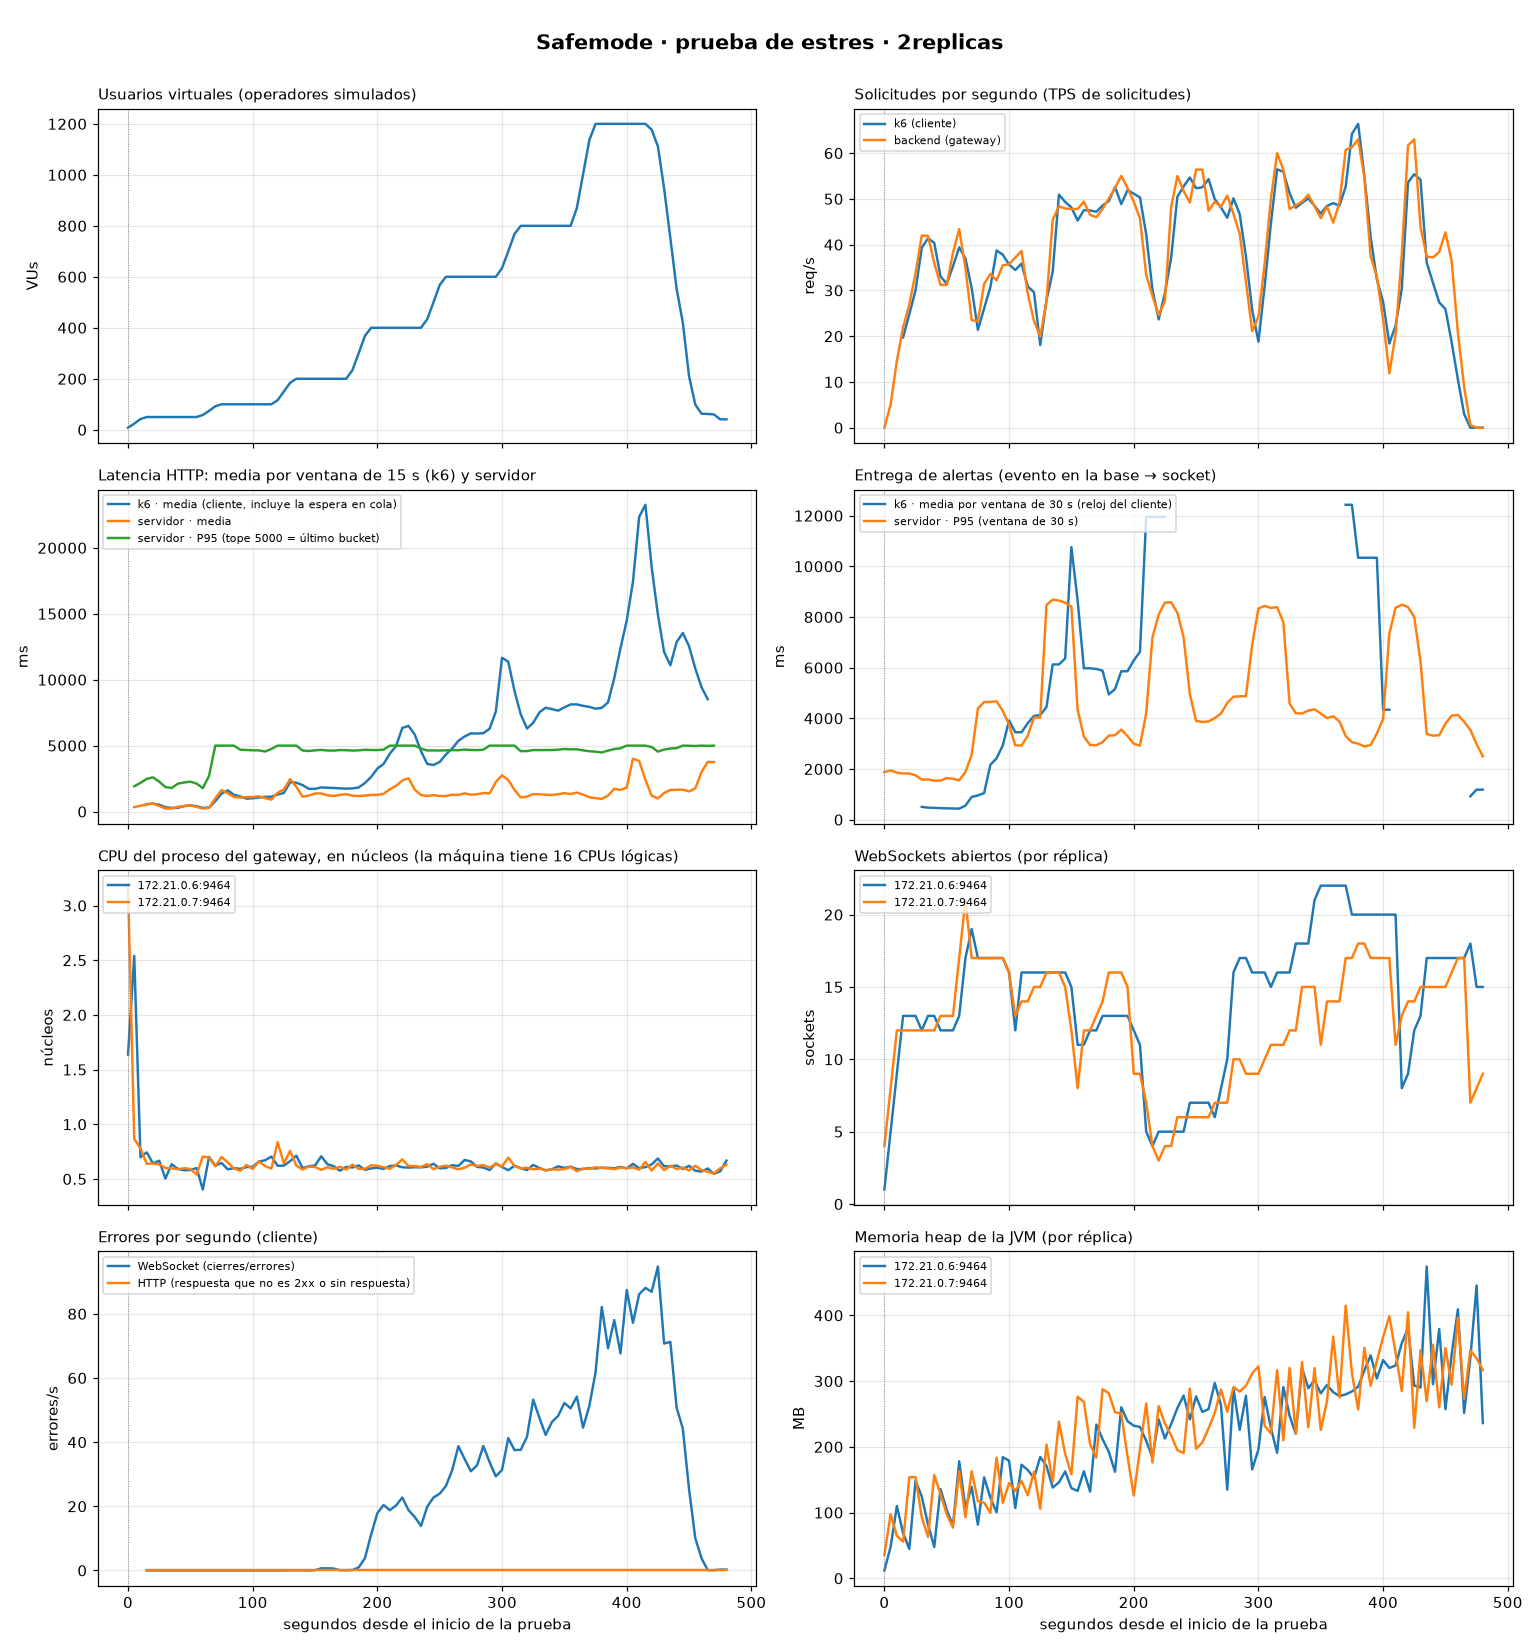
\includegraphics[width=0.96\textwidth,height=0.85\textheight,keepaspectratio]{../rendimiento/resultados/estres-2replicas/estres-2replicas.png}
\caption{Estrés con 2 réplicas \emph{antes} de la corrección: el TPS se aplana en torno a 40 req/s, la media del servidor se queda en 1~s y la del
cliente crece; la CPU del gateway no pasa de 0,7 núcleos.}\label{fig:estres-antes}
\end{figure}

\begin{figure}[p]
\centering
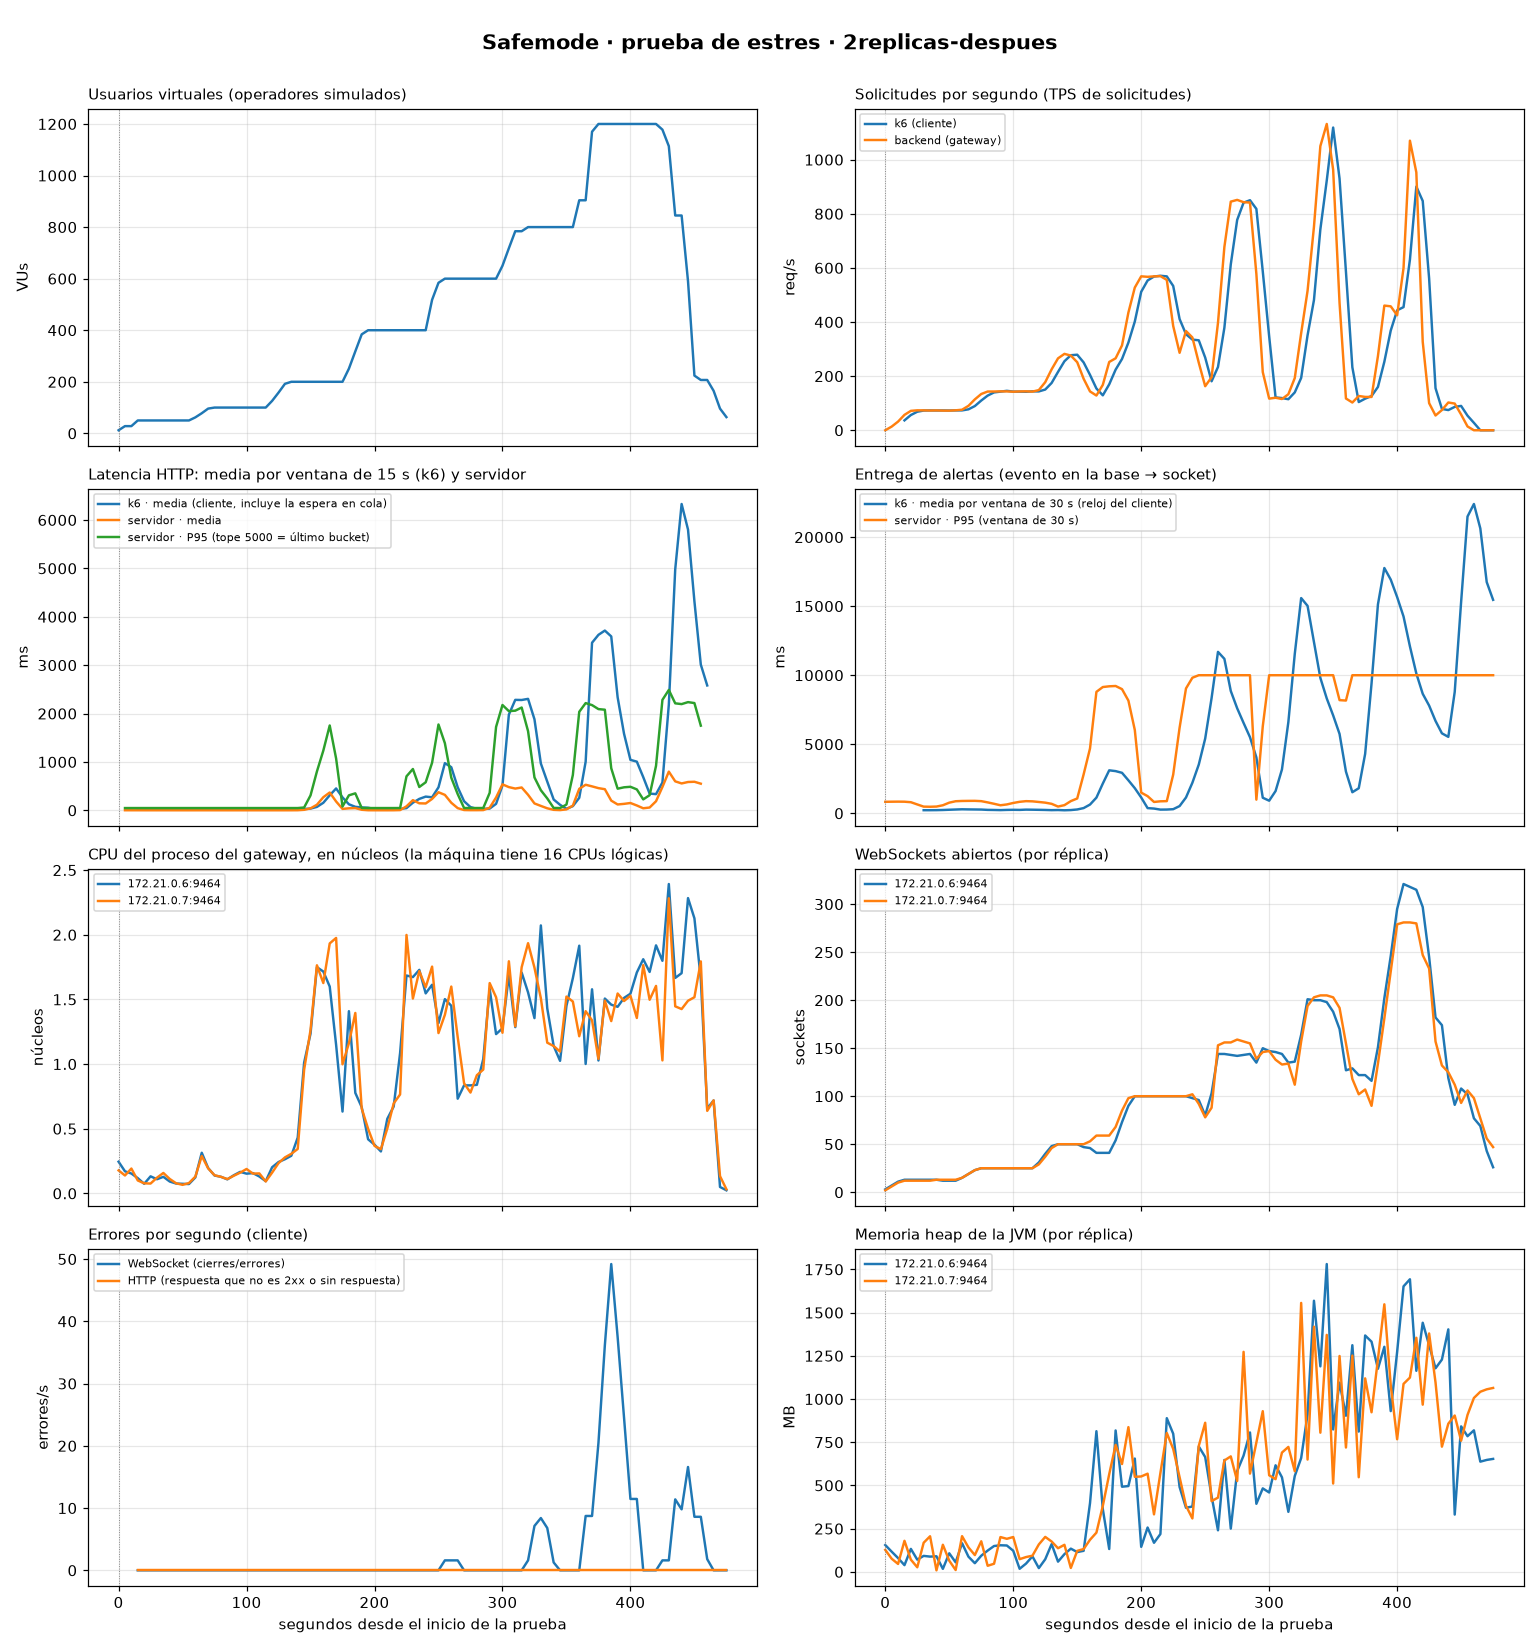
\includegraphics[width=0.96\textwidth,height=0.85\textheight,keepaspectratio]{../rendimiento/resultados/estres-2replicas-despues/estres-2replicas-despues.png}
\caption{Estrés con 2 réplicas \emph{después} de la corrección: HTTP llega a 678 req/s por escalón (picos de 1\,119 req/s), sin errores HTTP;
la entrega de alertas pasa a ser el límite.}\label{fig:estres-despues}
\end{figure}

% ------------------------------------------------------------------------------------------------------------------------------------
\section{Escalabilidad y disponibilidad}\label{sec:disponibilidad}

\begin{table}[H]
\centering\small
\caption{Escenario de disponibilidad y escalabilidad ED-1.}\label{tab:ed1}
\begin{tabularx}{\textwidth}{lY}
\toprule
\textbf{Fuente} & Un fallo interno: una réplica del gateway termina (error, falta de memoria o despliegue de una versión nueva) \\
\textbf{Estímulo} & Con operadores conectados y alertas llegando, una réplica deja de responder de golpe (SIGKILL) o termina sola \\
\textbf{Artefacto} & Capa de gateway (HTTP, WebSocket y motor de alertas) detrás del balanceador, con la base compartida \\
\textbf{Entorno} & Operación normal con carga continua y varios operadores con el panel abierto \\
\textbf{Respuesta} & El balanceador la excluye (vigilancia activa de \cod{/ready} y pasiva por conexión rechazada) y reintenta en la otra; los operadores se reconectan solos con la misma sesión; una alerta creada durante la caída llega a todos; la réplica se reinicia y vuelve \\
\textbf{Medida} & 0 peticiones fallidas; reconexión $\leq$ 2,1~s; 0 alertas perdidas o duplicadas; réplica de nuevo en rotación en $\approx$ 5~s \\
\bottomrule
\end{tabularx}
\end{table}

\textbf{Tácticas} \cite{bass}: detectar fallos (ping/echo sobre \cod{/ready}, que comprueba la base); recuperarse (redundancia activa de dos réplicas,
reintento, reinicio automático con \cod{restart: unless-stopped}); prevenir fallos (eliminar el estado local: las sesiones y las alertas viven
en la base, y cada réplica reconstruye lo que le falta).

\textbf{Qué se cambió en el código para poder escalar} (ADR~0006): (1) las alertas llegan a todas las réplicas porque cada una sondea la tabla
cada 0,5~s; (2) la creación de una alerta resiste la carrera entre réplicas (el \cod{UNIQUE} de la base decide y el SQLState 23505 se trata como
«ya existe»); y (3) las sesiones pueden guardarse en la base (\cod{SAFEMODE_SESSION_STORE=database}, con la huella SHA-256 del identificador y
falla cerrada), de modo que cualquier réplica reconoce la cookie que emitió otra.

\textbf{Cálculo de disponibilidad con los SLA publicados por AWS.} Hoy el despliegue público es un solo servidor y su disponibilidad es la de
una instancia EC2 (99,5\,\%, unas 3,6~h de caída al mes). El diseño objetivo (DNS $\rightarrow$ balanceador multi-AZ $\rightarrow$ dos gateways en
dos zonas $\rightarrow$ RDS Multi-AZ) llega a \textbf{99,9375\,\%} (3,2 «nueves», 27~min al mes), con la base de datos pesando el 80\,\% de la
indisponibilidad restante. Dos réplicas en el mismo servidor no mejoran nada: comparten instancia, zona y disco.

\begin{table}[H]
\centering\small
\caption{Prototipo de dos réplicas (tres corridas, 17/17 comprobaciones cada una; docs/disponibilidad/).}\label{tab:escalado}
\begin{tabularx}{\textwidth}{lY}
\toprule
\textbf{Medida} & \textbf{Resultado} \\
\midrule
Reparto de 30 peticiones con una sola sesión & 15 y 15 entre las réplicas; 30 de 30 con 200 \\
Caída de golpe (SIGKILL) con tráfico & \textbf{0 de 555 peticiones fallaron}; p50 45~ms, p99 250~ms \\
Reconexión de los operadores de la réplica caída & 2,07~s el más lento (2~s son la espera del panel) \\
Alerta creada durante la caída & 3 la recibieron en vivo y 3 al reconectar; ninguna perdida ni duplicada \\
Réplica de nuevo en rotación & 5,2~s si Docker la reinicia; 8,3~s si se arranca a mano \\
\bottomrule
\end{tabularx}
\end{table}

\textbf{Límite honesto.} 0 fallos en 555 peticiones solo permite afirmar, con 95\,\% de confianza, una disponibilidad de al menos 99,46\,\%
(regla de los tres): el prototipo mide el \emph{comportamiento ante fallos}, no la disponibilidad de largo plazo. Y el despliegue público sigue
siendo un servidor único: el despliegue distribuido en dos zonas está diseñado y calculado (Figura~\ref{fig:despliegue-objetivo}) pero no
desplegado, porque requiere recursos de AWS y una decisión de costo del equipo.

% ------------------------------------------------------------------------------------------------------------------------------------
\section{Seguridad}\label{sec:seguridad-resumen}
Tres escenarios, \textbf{aprobados por el docente}, con tácticas y validación ejecutable (capítulo~\ref{chap:seguridad}):
ES-1 autenticación y autorización del operador (35 pruebas), ES-2 protección frente a ataques web y revocación de sesión, y ES-3 integridad del
canal de imágenes \cod{/frames} (12 comprobaciones reproducibles). La sesión es una cookie de 256 bits \cod{HttpOnly} y \cod{SameSite=Strict}
de 12~h; el servidor guarda solo su huella SHA-256 y toda ruta protegida responde 401 sin sesión antes de ejecutar su manejador.

% ------------------------------------------------------------------------------------------------------------------------------------
\section{Portabilidad}\label{sec:portabilidad}

\begin{table}[H]
\centering\small
\caption{Escenario de portabilidad PT-1 (migración Cloud $\rightarrow$ On-Premise).}\label{tab:pt1}
\begin{tabularx}{\textwidth}{lY}
\toprule
\textbf{Fuente} & El equipo (o un cliente) que debe mover SafeMode de AWS a servidores propios \\
\textbf{Estímulo} & Decisión de migrar: no hay instancias EC2 ni servicios administrados de AWS disponibles \\
\textbf{Artefacto} & Todos los componentes: gateway, tracker, servicios de acceso y colaboración, bases de datos, proxy y observabilidad \\
\textbf{Entorno} & Un servidor Linux con Docker y Docker Compose, red local y dominio propio \\
\textbf{Respuesta} & Se clona el repositorio, se copia \cod{.env.example} a \cod{.env} con los valores propios y se levanta el mismo Compose; no hay cambios de código \\
\textbf{Medida} & 0 líneas de código cambiadas; todo componente se ejecuta en un contenedor o con una sola orden; la configuración sale solo de variables de entorno \\
\bottomrule
\end{tabularx}
\end{table}

\textbf{Evidencia.} Los componentes se empaquetan en contenedores (\cod{Dockerfile} por servicio) y el mismo conjunto de archivos Compose se
usa en tres entornos: el computador del desarrollador (Windows con Docker Desktop, donde corrieron todas las pruebas de este documento), el
prototipo de escalado y el servidor de AWS (\cod{docker-compose.publico.yml} con Caddy). La capa de datos se eligió sin dependencias de
proveedor: PostgreSQL, MongoDB y Redis en contenedores, y H2 como valor por defecto sin base externa; la única pieza propia de AWS es la
instancia que ejecuta Docker. El DNS (DuckDNS) y los certificados (Let's Encrypt, que gestiona Caddy) tampoco son de AWS. La guía
\cod{docs/despliegue/} y el script \cod{verificar-despliegue.ps1} comprueban el sitio publicado con peticiones de solo lectura.

\textbf{Qué cambiaría al migrar.} Solo lo operativo: el dominio y su DNS, la ruta del volumen de fotos, la rotación de claves y, si se
quiere alta disponibilidad, el balanceador (Caddy ya cumple ese papel en el prototipo) y la base replicada. \textbf{Límite declarado:} la
migración a un servidor on-premise distinto del equipo de desarrollo no se ejecutó como prueba; lo que se valida es que el mismo stack ya corre
en dos entornos distintos sin cambios.

% ------------------------------------------------------------------------------------------------------------------------------------
\section{Mantenibilidad}\label{sec:mantenibilidad}

\begin{table}[H]
\centering\small
\caption{Escenario de mantenibilidad MT-1 (inspección continua con análisis estático).}\label{tab:mt1}
\begin{tabularx}{\textwidth}{lY}
\toprule
\textbf{Fuente} & Una persona del equipo que sube un cambio al repositorio \\
\textbf{Estímulo} & \cod{git push} a cualquier rama o ejecución manual del workflow \\
\textbf{Artefacto} & Código fuente: backend Java (8 módulos Maven) y panel en JavaScript \\
\textbf{Entorno} & Integración continua en GitHub Actions, antes de cualquier despliegue \\
\textbf{Respuesta} & Compila, ejecuta las pruebas, mide la cobertura de cada capa y analiza estáticamente; si el control de calidad falla, el job falla y el despliegue no corre \\
\textbf{Medida} & Cobertura $\geq$ 80\,\% en backend y panel; fiabilidad, seguridad y mantenibilidad en A; control de calidad en verde \\
\bottomrule
\end{tabularx}
\end{table}

\textbf{Pipeline con reusable workflows.} \cod{pipeline.yml} llama a \cod{reusable-backend.yml} (\cod{mvn verify} con JaCoCo),
\cod{reusable-frontend.yml} (pruebas del panel con c8) y \cod{reusable-sonar.yml} (análisis con control de calidad), y el despliegue de la
EC2 depende de la calidad. La cobertura que se reporta es la de las pruebas que se ejecutan en esa corrida, no un número escrito a mano.

\begin{table}[H]
\centering\small
\caption{Resultados medidos (backend con JaCoCo; panel con c8; calificaciones con SonarQube Community 26.11 local).}\label{tab:mt-resultados}
\begin{tabularx}{\textwidth}{lYY}
\toprule
\textbf{Medida} & \textbf{Resultado} & \textbf{Meta} \\
\midrule
Cobertura de líneas del backend (479 pruebas) & 81,8\,\% (núcleo del producto 91,6\,\%) & $\geq$ 80\,\% \\
Cobertura del panel (144 pruebas, \cod{--all}) & 99,3\,\% de líneas & $\geq$ 80\,\% \\
Fiabilidad, seguridad, mantenibilidad & A, A, A (0 errores, 0 vulnerabilidades) & A \\
Control de calidad de Sonar & Verde; cobertura del código nuevo 98,5\,\% & Verde \\
Duplicación; olores de código & 0\,\%; 1 (no afecta calificación) & --- \\
\bottomrule
\end{tabularx}
\end{table}

\textbf{Lo que el análisis encontró.} Antes de la primera calificación había 4 errores y 4 «vulnerabilidades». Cuatro errores eran reales
(registros con arreglos que comparaban identidad, una expresión regular ambigua y un campo sin etiqueta) y se corrigieron con prueba. Las
cuatro «vulnerabilidades» de SQL formateado eran falsos positivos (solo reciben constantes del dialecto) y quedaron justificadas en el código.
Medir la cobertura del panel (41\,\% $\rightarrow$ 99\,\%) destapó además dos defectos reales de la interfaz. \textbf{Límites:} el script en
línea de \cod{index.html} no está medido; la corrida real en SonarCloud requiere la cuenta del equipo; y los adaptadores a bases de datos
(PostgreSQL, MongoDB, Redis) se prueban contra las bases reales fuera del pipeline.

% ------------------------------------------------------------------------------------------------------------------------------------
\section{Observabilidad}\label{sec:observabilidad}

\begin{table}[H]
\centering\small
\caption{Escenario de observabilidad OB-1.}\label{tab:ob1}
\begin{tabularx}{\textwidth}{lY}
\toprule
\textbf{Fuente} & Un operador del sistema (o el docente) que necesita saber si SafeMode funciona y por qué se degrada \\
\textbf{Estímulo} & Una dependencia cae (PostgreSQL, Redis, el servicio de acceso) o la latencia sube bajo carga \\
\textbf{Artefacto} & Métricas de aplicación y de dependencias; Prometheus; Grafana; reglas de alerta \\
\textbf{Respuesta} & El tablero muestra tráfico, latencia, errores, CPU, memoria y estado de cada dependencia; una regla de Prometheus se dispara y dice qué hacer \\
\textbf{Medida} & La degradación se detecta en $\leq$ 1~min (\cod{for: 1m}); cada dependencia publica \cod{safemode_dependency_up} (1 sirve, 0 cae) \\
\bottomrule
\end{tabularx}
\end{table}

\textbf{Qué se instrumentó.} El gateway publica métricas con Micrometer en el puerto 9464 (tráfico, latencia y errores por ruta
\cod{safemode_http_request_seconds}, entrega de alertas \cod{safemode_alert_delivery_seconds}, sockets abiertos, alertas por severidad y tipo, y
el estado de la base como dependencia); los servicios de acceso y colaboración publican las suyas. Prometheus recoge cada réplica por DNS, y Grafana
muestra el tablero del equipo (\cod{observability/dashboards/dashboard-safemode-v2.json}) junto con los de persistencia. k6 envía sus métricas a
Prometheus por \emph{remote write}, de modo que las pruebas de carga se ven en el mismo tablero antes, durante y después.

\textbf{Condiciones de degradación detectables.} Ocho reglas (\cod{performance/monitoring/reglas-alertas.yml}, validadas con \cod{promtool}):
gateway caído, base inaccesible, réplica no lista, latencia HTTP alta, entrega de alertas lenta, errores 5xx, CPU alta y demasiados sockets. En las
pruebas se dispararon las de \textbf{latencia} y de \textbf{entrega}; la de CPU no, porque el cuello de botella no era la CPU: una enseñanza
útil, pues vigilar solo el recurso habría dado una falsa tranquilidad. \textbf{Pendiente:} la captura del tablero con el período de una prueba.

% ------------------------------------------------------------------------------------------------------------------------------------
\section{Robustez en concurrencia y tiempo real}\label{sec:concurrencia}

\begin{table}[H]
\centering\small
\caption{Escenario de concurrencia CO-1 (laboratorio de consistencia, ADR~0005).}\label{tab:co1}
\begin{tabularx}{\textwidth}{lY}
\toprule
\textbf{Fuente} & Dos operadores que editan a la vez la configuración del puesto; una dependencia que cae a mitad de una operación \\
\textbf{Estímulo} & Dos escrituras con la misma versión; una revocación de permiso; Redis o el servicio de acceso detenidos \\
\textbf{Respuesta} & Una escritura gana (200) y la otra recibe 409; se rechaza la escritura de quien perdió el permiso (403); si no se puede verificar el permiso, no se guarda (503) \\
\textbf{Medida} & Antes: dos 200 y una edición perdida; después: [200, 409] y revocado 403 con el documento intacto; 4 de 4 comprobaciones \\
\bottomrule
\end{tabularx}
\end{table}

\textbf{Mecanismos.} La versión viaja \emph{en el filtro} de la misma operación atómica de MongoDB (\cod{findOneAndUpdate}), de modo que no hay
ventana entre leer y escribir; el permiso se pregunta siempre a la autoridad (PostgreSQL) y la caché de Redis solo sirve para pintar la
pantalla, nunca para autorizar; la presencia y el permiso en caché se guardan con su vencimiento en una sola escritura (\cod{SET ... EX}).
En el producto, una alerta es única por evento aunque haya varios paneles o réplicas (\cod{UNIQUE} en la base), y dos cámaras se analizan en
paralelo con un seguimiento independiente por cámara. \textbf{Límite declarado:} PostgreSQL y MongoDB no comparten transacción, por lo que
entre validar el permiso y guardar queda una ventana pequeña; la alternativa (PostgreSQL con JSONB) está explicada en el ADR.

\chapter{Vista de arquitectura}

\section{Estilo arquitectónico}
SafeMode combina cuatro estilos, cada uno aplicado donde resuelve un problema concreto (los diagramas de los capítulos siguientes lo muestran):

\begin{description}[leftmargin=1.2em,style=nextline]
  \item[Tuberías y filtros (\emph{pipes and filters}) en el procesamiento de imagen.] El fotograma recorre etapas que no conocen a la
  siguiente: fuente de fotogramas $\rightarrow$ detector YOLOv8 $\rightarrow$ seguimiento de objetos y personas $\rightarrow$ almacén de
  eventos. Cada etapa se puede probar y reemplazar por separado (por ejemplo, la fuente de imagen por captura de pantalla o por la ventana
  compartida desde el navegador implementan la misma interfaz \cod{FrameSource}).
  \item[Orientado a eventos con difusión (\emph{publish/subscribe}) para las alertas.] El motor de alertas lee los retiros nuevos y avisa a
  los oyentes registrados (\cod{addListener}): el servidor WebSocket y el servicio de avisos. Agregar un canal nuevo no toca el motor.
  \item[Cliente--servidor con empuje en tiempo real.] El panel web (página estática sin \emph{build}) es el cliente; el gateway le entrega
  la página, las fotos y la API HTTP, y le \emph{empuja} las alertas por WebSocket sin que tenga que preguntar.
  \item[Servicios pequeños con persistencia políglota para el estado compartido.] El servicio de acceso (permisos, PostgreSQL) y el de
  colaboración (configuración del puesto, MongoDB; presencia y caché, Redis) son procesos aparte porque tienen garantías distintas que
  defender (ADR~0005).
\end{description}

\textbf{Por qué no microservicios para todo.} El núcleo del producto es un reactor Maven de módulos con un solo proceso de gateway (que
contiene el motor de alertas y el servicio de avisos) y un tracker aparte. Un equipo de tres personas y un requisito de menos de 5~s
de extremo a extremo favorecen pocos procesos y llamadas locales; lo que escala por operadores (el gateway) se hizo \emph{sin estado}
para poder replicarlo (ADR~0006), y lo que no se debe replicar (el tracker, por cámara, junto a la pantalla y los modelos) quedó aparte. La
frontera entre procesos está donde cambian las garantías o la forma de escalar, no por moda.

\section{Modelo cloud}
El despliegue público usa el modelo de \textbf{infraestructura como servicio (IaaS)}: una instancia EC2 de AWS que ejecuta Docker, con todos
los componentes en contenedores y las bases de datos autoadministradas en contenedores. Se evitó a propósito depender de servicios
administrados propios de un proveedor (la portabilidad, sección~\ref{sec:portabilidad}). Los servicios de terceros se consumen como
\textbf{SaaS}: Google Identity Services (identidad), Telegram (avisos) y, de forma opcional, el servicio de visión de NVIDIA. El diseño
objetivo de disponibilidad añade servicios administrados de AWS (balanceador, RDS Multi-AZ y DNS), documentado pero no desplegado.

\section{Decisiones clave}
Cada decisión importante tiene un registro (ADR) con alternativas y consecuencias en \cod{docs/adr/}. La Tabla~\ref{tab:adr} las resume.

\begin{table}[H]
\centering\small
\caption{Decisiones de arquitectura (ADR).}\label{tab:adr}
\begin{tabularx}{\textwidth}{lYY}
\toprule
\textbf{ADR} & \textbf{Decisión} & \textbf{Por qué / consecuencia} \\
\midrule
0001 & Un \cod{Dockerfile} por módulo, con el reactor Maven como contexto; Xvfb para que AWT inicie sin pantalla & Los módulos comparten el \cod{pom} padre; se probó en Docker Desktop real, no solo por razonamiento \\
0002 & El gateway en un contenedor con el motor dentro (misma JVM); H2 en modo servidor; la conexión por \cod{SAFEMODE_DB_URL}; puertos solo en 127.0.0.1 & Sin la variable todo funciona como antes (H2 local); la base y las fotos tienen datos de personas y no se exponen \\
0003 & Dos cámaras desde una ventana compartida del navegador; zonas dibujadas con prueba previa; un seguimiento por cámara; reporte; «dueño que volvió» & Mediciones: yolov8m 371~ms con 1 cámara; con 2 cámaras yolov8s con 8 hilos por detector. La ventana de cámaras no puede minimizarse (límite del sistema operativo) \\
0004 & Login con Google verificado en el servidor, lista blanca, sesión por cookie; avisos de texto por navegador y Telegram & Solo texto, sin fotos ni datos de personas, en aviso externo; el correo no se implementó \\
0005 & PostgreSQL, MongoDB y Redis, cada uno por lo que garantiza; caché solo para mostrar, nunca para autorizar & Edición perdida resuelta con la versión en el filtro; falla cerrada si la autoridad no responde \\
0006 & Gateway sin estado y replicable; alertas por sondeo de la base; sesiones compartidas opcionales; balanceador con vigilancia activa y pasiva & No hay afinidad de sesión; la base decide la unicidad de la alerta (\cod{UNIQUE}) \\
\bottomrule
\end{tabularx}
\end{table}

\textbf{Decisiones transversales.} (1) \emph{Configuración por entorno:} todo valor que varía (claves, URL de la base, orígenes) llega por
variable de entorno, nunca por código ni repositorio. (2) \emph{Fallar cerrado:} ante la duda, se deniega (sesión sin base de datos, permiso sin
autoridad, valor desconocido de una variable de configuración). (3) \emph{Lo que ya funciona no se rompe:} las capacidades nuevas son opcionales y
con valor por defecto igual al comportamiento anterior (por ejemplo, H2 por defecto y PostgreSQL con una URL).

\section{Justificación del balanceo, el despliegue distribuido y los servicios en tiempo real}
\textbf{Balanceo.} Solo la capa de gateway escala por número de operadores; por eso es la única que se replica. El balanceador reparte sin
afinidad de sesión (las sesiones están en la base) y vigila cada réplica con \cod{/ready}, que comprueba que llegue a la base; una réplica
viva pero sin base no recibe tráfico. En el prototipo el balanceador es Caddy; en AWS sería un Application Load Balancer (Figura~\ref{fig:despliegue-objetivo}).

\textbf{Despliegue distribuido.} Varios contenedores en un solo equipo no reemplazan un despliegue distribuido, y por eso el documento es
explícito: el servidor público es único (Figura~\ref{fig:despliegue-actual}); el diseño distribuido (dos zonas, base administrada Multi-AZ) se calculó
con los SLA publicados (99,5\,\% $\rightarrow$ 99,9375\,\%) y su comportamiento se validó con el prototipo de dos réplicas, pero no se desplegó. Se
eligió ese reparto porque la base de datos es el límite (80\,\% de la indisponibilidad restante); Redis, MongoDB y el servicio de acceso quedan
\emph{fuera del camino crítico} de una alerta y no se replican en esta etapa. El tracker es un punto único de \emph{detección} que ningún SLA de
la nube cubre: corre por cámara, en el borde, y se mitiga solo con reinicio automático.

\textbf{Servicios en tiempo real.} La promesa de valor es avisar en menos de 5~s. El camino de una alerta (Figura~\ref{fig:secuencia-alerta})
evita todo lo que sume latencia: el tracker escribe el evento en la base, el motor lo lee cada 1~s, y el WebSocket lo empuja a los paneles
(medido: del evento al panel, media 0,5~s y P95 0,9~s); los avisos externos salen en hilos aparte para que un canal lento no retrase la alerta;
y la ruta crítica no depende de Redis, MongoDB ni del servicio de acceso. Cada WebSocket exige sesión y \cod{Origin} del panel, y el servidor
revalida la sesión en cada mensaje y cierra los sockets de sesiones terminadas.

\chapter{Diagramas de arquitectura}

\section{Notación y fuente de los diagramas}
Los diagramas se modelaron en \textbf{ArchiMate} con la herramienta Archi, en un solo modelo versionado
(\cod{docs/diagramas/safemode-arquitectura.archimate}); las figuras de este capítulo son las vistas 4 a 16 de ese modelo, exportadas con Archi
en línea de comandos (\cod{docs/arquitectura/exportar-vistas.py}). Describen \textbf{lo implementado}: cada puerto, ruta, clase, tabla y servicio
se verificó contra el código. Las tres vistas anteriores del equipo (1 a 3, de la etapa de diseño) siguen en el modelo como historia.

ArchiMate no trae la notación UML, así que cada tipo de diagrama que pide el requerimiento se expresa con los elementos que el estándar sí
tiene. La Tabla~\ref{tab:uml} dice cuál vista cubre cada uno y cómo se lee.

\begin{table}[H]
\centering\small
\caption{Diagramas requeridos y la vista ArchiMate que los cubre.}\label{tab:uml}
\begin{tabularx}{\textwidth}{lllY}
\toprule
\textbf{Diagrama} & \textbf{Vista} & \textbf{Figura} & \textbf{Cómo se expresa en ArchiMate} \\
\midrule
Contexto & 4 & \ref{fig:contexto} & El sistema como un componente de aplicación rodeado de actores y sistemas externos (en gris) \\
Componentes & 5 y 6 & \ref{fig:comp-flujo}, \ref{fig:comp-puesto} & Componentes de aplicación con composición (partes de un proceso) y flujos entre ellos \\
Clases & 7, 8 y 9 & \ref{fig:clases-1}--\ref{fig:clases-3} & Cada clase es un componente; \emph{Realization} = implementa la interfaz; \emph{Composition} = contiene; \emph{Serving} = presta servicio a \\
Entidad-relación & 10 & \ref{fig:er} & Objetos de datos (tablas, documentos, claves) con asociaciones N:1 \\
Secuencia & 11 y 12 & \ref{fig:secuencia-alerta}, \ref{fig:secuencia-login} & Vista dinámica: componentes y flujos numerados en el orden de la interacción \\
Despliegue & 13 y 14 & \ref{fig:despliegue-actual}, \ref{fig:despliegue-objetivo} & Nodos, software de sistema y redes de la capa de tecnología \\
Actividades & 15 y 16 & \ref{fig:act-1}, \ref{fig:act-2} & Procesos con relaciones de disparo, eventos y uniones (O = decisión; Y = unión) \\
\bottomrule
\end{tabularx}
\end{table}

\textbf{Convenciones.} Gris = sistema externo o fuera de nuestro control; azul = capa de aplicación; verde = tecnología; amarillo =
negocio; naranja (Figura~\ref{fig:despliegue-objetivo}) = diseñado y calculado pero \emph{no desplegado}. Las líneas punteadas con flecha son
flujos; las continuas con rombo, composición.

\section{Contexto}
El sistema se ve como una sola pieza rodeada de quienes lo usan y de los sistemas con los que habla. El personal de seguridad y el administrador
reciben servicio del sistema; las cámaras se ven en el software de cámaras (VMS), cuya ventana compartida es la entrada de imagen; Google
verifica la identidad; Telegram recibe avisos de texto; el servicio de visión de NVIDIA es opcional; y GitHub Actions y SonarCloud
despliegan y analizan el código. El video no se guarda en SafeMode.

\vista{04-contexto.png}{Contexto del sistema (vista 4).}{fig:contexto}

\section{Componentes}
La Figura~\ref{fig:comp-flujo} sigue el camino de una alerta: el panel recibe la ventana del VMS y envía un fotograma por cámara al
\emph{Camera Feed}; el detector produce detecciones que el seguimiento convierte en eventos (y fotos); el motor de alertas, dentro del gateway,
lee los retiros nuevos, crea la alerta y la entrega al servidor WebSocket y al servicio de avisos. El gateway tiene seis partes (composición) y
lanza el tracker con un comando fijo. La Figura~\ref{fig:comp-puesto} muestra el Release~2: el puesto compartido (zonas, historial y presencia) en
\emph{collaboration-service}, los permisos en \emph{access-service} (que la colaboración consulta antes de cada escritura y que falla cerrada), los
tres motores de datos y la observabilidad.

\vista{05-componentes-flujo.png}{Componentes: de la cámara a la alerta (vista 5).}{fig:comp-flujo}
\vista{06-componentes-puesto.png}{Componentes: puesto compartido, permisos y observabilidad (vista 6).}{fig:comp-puesto}

\section{Clases}
Se muestran las clases que sostienen las decisiones de diseño, en tres vistas. La primera (Figura~\ref{fig:clases-1}): el
\cod{ObjectTracker} (uno por cámara) contiene objetos y personas seguidos, usa descriptores de apariencia y una huella de la zona para
verificar un retiro, y delega la descripción por IA en una interfaz que implementa el cliente de NVIDIA. La segunda (Figura~\ref{fig:clases-2}):
los almacenes de eventos y alertas comparten conexión con reconexión automática y dialecto (H2 o PostgreSQL), y el motor de alertas combina
eventos y reglas para crear alertas únicas que avisa a sus oyentes. La tercera (Figura~\ref{fig:clases-3}): el \cod{GatewayRunner} arma el
servidor HTTP, el WebSocket, la autenticación y el servicio de avisos; la sesión y la verificación del token son interfaces con dos
implementaciones (memoria o base) y una (Google), lo que permitió replicar el gateway sin cambiar su código.

\vista{07-clases-deteccion.png}{Clases (1/3): detección y seguimiento (vista 7).}{fig:clases-1}
\vista{08-clases-persistencia.png}{Clases (2/3): persistencia y motor de alertas (vista 8).}{fig:clases-2}
\vista{09-clases-gateway.png}{Clases (3/3): gateway, sesiones y avisos (vista 9).}{fig:clases-3}

\section{Entidad-relación}
El modelo de datos tiene cuatro grupos. En la base de eventos (H2 por defecto, PostgreSQL con una URL): \cod{object_presence_event} y
\cod{alert} (una alerta por evento, garantizada por \cod{UNIQUE}), \cod{camera} y \cod{operator_session} (la huella SHA-256 de la cookie, nunca la
cookie). En PostgreSQL de acceso: puestos, operadores, membresías (rol y permiso de configurar) y auditoría de concesiones y revocaciones. En MongoDB:
el documento del puesto con su versión y el historial de cambios (índice único por puesto y versión, retención de 90 días). En Redis: presencia y
caché de permisos, con vencimiento.

\vista{10-entidad-relacion.png}{Modelo de datos: tablas, documentos y claves (vista 10).}{fig:er}

\section{Secuencia}
La primera secuencia (Figura~\ref{fig:secuencia-alerta}) es la promesa de valor: del retiro de un objeto al aviso en el panel en menos de
5~s, con el presupuesto de tiempo anotado. La segunda (Figura~\ref{fig:secuencia-login}) es el inicio de sesión con Google: el ID token se
verifica en el servidor (se le pregunta a Google y se comprueban emisor, audiencia y vigencia), el correo debe estar en la lista blanca, la sesión se guarda por su huella y el
navegador recibe una cookie \cod{HttpOnly}; el WebSocket revalida la sesión.

\vista{11-secuencia-alerta.png}{Secuencia: del retiro de un objeto al aviso en el panel (vista 11).}{fig:secuencia-alerta}
\vista{12-secuencia-login.png}{Secuencia: inicio de sesión con Google (vista 12).}{fig:secuencia-login}

\section{Despliegue}
La Figura~\ref{fig:despliegue-actual} es el despliegue público de hoy: una instancia EC2 que ejecuta Docker Compose con Caddy delante (TLS,
\cod{forward_auth} para \cod{/frames} y \cod{/grafana}) y todos los servicios detrás; un solo servidor, por lo que su caída es total. La
Figura~\ref{fig:despliegue-objetivo} pone lado a lado el \textbf{prototipo validado} (dos réplicas detrás de un balanceador con PostgreSQL, medido en
la sección~\ref{sec:disponibilidad}) y el \textbf{diseño objetivo} en AWS (Route~53, balanceador multi-AZ, dos instancias en zonas distintas y RDS
Multi-AZ), señalado como no desplegado.

\vista{13-despliegue-actual.png}{Despliegue actual: servidor único en AWS con Docker Compose (vista 13).}{fig:despliegue-actual}
\vista{14-despliegue-objetivo.png}{Prototipo de escalado validado y diseño objetivo en AWS (vista 14).}{fig:despliegue-objetivo}

\section{Actividades}
El flujo se parte en dos. En la Figura~\ref{fig:act-1}, cada fotograma se detecta y se empareja con lo ya seguido; un objeto se registra cuando lleva 3~s
quieto; y se da por retirado si desaparece 3 fotogramas o se desplaza más de 25~px en 2 seguidos, siempre que la verificación por imagen
(huella de 24$\times$24 puntos, sin contar a las personas que tapan) confirme que cambió. En la Figura~\ref{fig:act-2}, el retiro se clasifica
según quién estaba cerca y se traduce a una alerta de severidad alta, media o baja; la alerta se crea una sola vez, se publica a todos los
operadores y, si es alta o media, sale el aviso de texto.

\vista{15-actividades-retiro.png}{Actividades (1/2): del fotograma al retiro confirmado (vista 15).}{fig:act-1}
\vista{16-actividades-alerta.png}{Actividades (2/2): del retiro a la alerta y el aviso (vista 16).}{fig:act-2}

\chapter{Detalles tecnológicos}

\section{Lenguajes y frameworks}
\begin{table}[H]
\centering\small
\caption{Tecnologías por capa (versiones tomadas de los pom.xml y de los archivos Compose).}\label{tab:tec}
\begin{tabularx}{\textwidth}{lYY}
\toprule
\textbf{Capa} & \textbf{Tecnología} & \textbf{Para qué} \\
\midrule
Backend & Java 17 (Temurin), Maven (reactor de 8 módulos) & Detección, seguimiento, alertas, gateway y servicios de apoyo \\
Visión & YOLOv8 exportado a ONNX; ONNX Runtime 1.18.0 & Detectar personas y maletas; estimar la pose del dueño (YOLOv8-pose) \\
Tiempo real & Java-WebSocket 1.5.6; servidor HTTP del JDK con pool de 32 hilos & Empujar alertas; servir panel, fotos y API \\
Datos & H2 2.2.224 (por defecto); PostgreSQL 16.6 (JDBC 42.7.4, HikariCP en el servicio de acceso); MongoDB 7.0.16 (controlador 5.2.1); Redis 7.4.2 (Jedis 5.2.0) & Eventos y alertas; permisos; configuración compartida y su historial; presencia y caché \\
Serialización & Gson 2.11.0 & Mensajes JSON del WebSocket y de la API \\
Panel & HTML, CSS y JavaScript sin \emph{build}; pruebas con Node, jsdom y c8 & Tablero de alertas en vivo, compartir ventana, zonas, reporte \\
Métricas & Micrometer 1.13.6 (registro de Prometheus) & Tráfico, latencia, entrega de alertas y dependencias \\
Pruebas & JUnit 5.10.2; JaCoCo 0.8.14; k6 0.57.0 & Unitarias y de integración; cobertura; carga, estrés y pico \\
\bottomrule
\end{tabularx}
\end{table}

\section{Infraestructura y servicios}
\begin{itemize}
  \item \textbf{Nube:} una instancia EC2 de AWS (AWS Academy Learner Lab); el dominio es \cod{safemode-arsw.duckdns.org} (DuckDNS) y el certificado
  TLS lo obtiene y renueva Caddy con Let's Encrypt.
  \item \textbf{Proxy:} Caddy 2.8 como única entrada pública: \cod{/ws} al WebSocket, \cod{/frames} y \cod{/grafana} detrás de \cod{forward_auth}
  contra \cod{/auth/me}, y el resto al panel.
  \item \textbf{Servicios de terceros:} Google Identity Services (OpenID Connect), la API de bots de Telegram y, de forma opcional, el modelo de
  visión de NVIDIA (el modelo por defecto es un Nemotron sin razonamiento, tras retirarse el anterior).
  \item \textbf{Almacenamiento de evidencia:} fotos PNG en un volumen; la base guarda solo la ruta.
\end{itemize}

\section{DevOps y CI/CD}
El pipeline (\cod{.github/workflows/pipeline.yml}) corre en cada \cod{push} y se compone de \emph{reusable workflows}:

\begin{table}[H]
\centering\small
\caption{Etapas del pipeline.}\label{tab:pipeline}
\begin{tabularx}{\textwidth}{lYY}
\toprule
\textbf{Etapa} & \textbf{Workflow} & \textbf{Qué hace} \\
\midrule
Backend & \cod{reusable-backend.yml} & Java 17, \cod{mvn -B verify}: compila, prueba y mide la cobertura con JaCoCo; sube los informes \\
Frontend & \cod{reusable-frontend.yml} & Node 24, \cod{npm ci}, pruebas del panel con cobertura (c8, \cod{--all}); sube \cod{lcov.info} \\
Quality & \cod{reusable-sonar.yml} & Descarga ambos informes y analiza con SonarCloud; falla si el control de calidad no pasa \\
Deploy & job \cod{deploy} & Despliegue por SSH a la EC2 en \cod{develop} y \cod{main}, con una comprobación posterior de que el panel responde \\
\bottomrule
\end{tabularx}
\end{table}

La etapa de calidad se omite con un aviso (sin romper) mientras el equipo no configure el token y las variables de SonarCloud; con todo
configurado, falla si el control no pasa y, como el despliegue depende de ella, un cambio que no cumple no llega al servidor.

\section{Docker y Docker Compose}
Cada módulo tiene su \cod{Dockerfile}; los archivos Compose se combinan por capas (\cod{-f} varias veces) en lugar de duplicarse:

\begin{table}[H]
\centering\small
\caption{Archivos Compose y su papel.}\label{tab:compose}
\begin{tabularx}{\textwidth}{lY}
\toprule
\textbf{Archivo} & \textbf{Papel} \\
\midrule
\cod{docker-compose.yml} & Base: captura de imagen, visión, base H2 en modo servidor y gateway; proyecto \cod{safemode-arsw} \\
\cod{docker-compose.persistencia.yml} & PostgreSQL, MongoDB, Redis, servicios de acceso y colaboración, Prometheus, Grafana, sonda \cod{/ready} y k6 \\
\cod{docker-compose.tracker.yml} & El tracker en un contenedor (despliegue público) \\
\cod{docker-compose.publico.yml} & Caddy como entrada pública y reinicio automático de los servicios \\
\cod{docker-compose.escalado.yml} & Prototipo de escalado: balanceador Caddy y réplicas del gateway (proyecto \cod{safemode-escalado}, aparte del normal) \\
\cod{docker-compose.sonar.yml} & SonarQube local para ver las calificaciones antes del pipeline \\
\bottomrule
\end{tabularx}
\end{table}

\section{Prometheus, Grafana y k6}
Prometheus (5~s de \emph{scrape} y de evaluación de reglas) descubre cada réplica del gateway por DNS y también recoge los servicios de acceso
y colaboración y la sonda \cod{/ready}; Grafana muestra el tablero del equipo y los de persistencia (13.3.1, porque el formato v2 del tablero no
carga en la 11.5); y k6 corre en un contenedor y envía sus métricas a Prometheus por \emph{remote write}. Los scripts de k6
(\cod{performance/k6/safemode.js}), el ejecutor que levanta el prototipo y deja la base en un estado conocido
(\cod{performance/ejecutar.ps1}), el generador de gráficas (\cod{performance/graficar.py}) y las reglas de alerta quedan versionados y son
reproducibles. Las gráficas calculan la latencia del cliente por ventana a partir de los contadores de k6 (porque k6 exporta sus percentiles
acumulados) y se verificaron contra el resumen de k6: misma media, mismas solicitudes, mismas alertas y mismos errores.

\chapter{Seguridad del sistema}\label{chap:seguridad}

\section{Autenticación y autorización}
\textbf{Autenticación.} El operador entra con su cuenta de Google (OpenID Connect). El navegador entrega el ID token; el servidor lo verifica
preguntándole a Google (endpoint \cod{tokeninfo}) y comprueba emisor, audiencia (el ID de cliente del proyecto), vigencia y correo verificado.
Nunca se guardan contraseñas: las maneja Google.

\textbf{Autorización.} Solo entra quien está en la lista blanca de correos (\cod{SAFEMODE_ALLOWED_EMAILS}); una cuenta válida pero ajena recibe
403 y ninguna cookie. Los roles (administrador, operador, lector) y el permiso de configurar viven en el servicio de acceso (PostgreSQL, con
auditoría de concesiones y revocaciones); toda escritura del puesto pregunta a esa autoridad en el momento y, si no responde, se deniega.

\textbf{Sesión.} Un identificador aleatorio de 256 bits va en una cookie \cod{HttpOnly} y \cod{SameSite=Strict} de 12~h; el servidor
conserva solo su huella SHA-256 (memoria o base), de modo que ni un volcado de la base permite reutilizarla, y es opaca: no hay token firmado
que robar tras cerrar sesión. La sesión protege toda la superficie: página, fotos, reporte, botones del tracker y el WebSocket, que además se
cierra (código 1008) cuando su sesión termina.

\section{Cifrado}
El tráfico del despliegue público va cifrado con TLS: Caddy obtiene y renueva el certificado de Let's Encrypt y es la única entrada
(el resto de los servicios se publican solo en \cod{127.0.0.1}). Las contraseñas y las claves no se guardan en el repositorio. Del cifrado en
reposo: las fotos y las bases residen en volúmenes del servidor sin cifrado propio de la aplicación. \textbf{Brecha declarada:} la cookie
de sesión no lleva el atributo \cod{Secure}.

\section{Buenas prácticas}
\begin{itemize}
  \item \textbf{Secretos solo en variables de entorno}: ID de cliente de Google, lista de correos, token del bot de Telegram, clave de NVIDIA,
  claves internas; el repositorio trae solo \cod{.env.example}. Los registros y los mensajes de error no llevan las claves.
  \item \textbf{Fallar cerrado}: sin base de datos no hay sesión; sin autoridad no se guarda; un valor desconocido de la configuración impide arrancar.
  \item \textbf{Validar toda entrada}: identificadores acotados, cuerpos limitados, rutas de fotos solo por nombre dentro de su carpeta, \cod{Origin} y
  \cod{Host} exigidos a toda petición que cambia estado (CSRF y DNS \emph{rebinding}).
  \item \textbf{Privacidad por diseño}: no se guarda video; los avisos externos son solo texto, sin fotos ni datos de personas; la descripción por IA
  externa es opcional y está declarada.
  \item \textbf{Revisión de seguridad} del código del gateway y del panel (solo lectura, perfil rápido): cinco pistas, cuatro reproducidas con
  pruebas y corregidas; la quinta sigue abierta y solo importa en un equipo compartido.
\end{itemize}

\section{Evidencias de los tres escenarios aprobados}
Los tres escenarios de seguridad fueron presentados al docente y \textbf{aprobados}. Cada uno trae un comando que comprueba su medida
(\cod{docs/seguridad/escenarios-de-seguridad.md}).

\begin{table}[H]
\centering\small
\caption{Escenarios de seguridad ES-1 a ES-3.}\label{tab:es}
\begin{tabularx}{\textwidth}{lYYY}
\toprule
 & \textbf{ES-1 Autenticación y autorización} & \textbf{ES-2 Ataques web y ciclo de la sesión} & \textbf{ES-3 Integridad de \cod{/frames}} \\
\midrule
\textbf{Estímulo} & Persona sin cuenta o con una cuenta válida pero no autorizada intenta abrir panel, fotos, WebSocket o configuración &
Página hostil abierta, enlace con \cod{?ws=}, conexión retenida o sesión que ya terminó &
Atacante sin cuenta envía imágenes falsas al canal de frames \\
\textbf{Tácticas} & Identificar, autenticar y autorizar actores; limitar acceso & Limitar acceso y exposición; revocar acceso; limitar el efecto de conexiones retenidas & Autenticar y limitar acceso en el proxy (\cod{forward_auth}) \\
\textbf{Medida} & 100\,\% de rutas protegidas $\rightarrow$ 401 sin sesión; fuera de la lista $\rightarrow$ 403 sin cookie; 0 fotos sin sesión &
0 cambios desde un origen ajeno; con una conexión retenida otro cliente se atiende en 5 a 288~ms; tras cerrar sesión, 0 alertas al socket abierto &
100\,\% de conexiones sin sesión $\rightarrow$ 401; 0 frames de no autenticados llegan al detector \\
\textbf{Evidencia} & 4 clases de prueba, 35 pruebas JUnit & 4 clases de prueba JUnit y pruebas del panel; verificación manual en Chrome & Script reproducible con Caddy y el receptor reales: 12 de 12 comprobaciones \\
\textbf{Estado} & Implementado & Implementado & Implementado; falta redesplegar \\
\bottomrule
\end{tabularx}
\end{table}

\textbf{Hallazgo que motivó ES-3.} El receptor de frames solo rechaza un \cod{Origin} \emph{presente} y distinto: un cliente que no lo manda, o
lo falsifica, inyectaba imágenes, y el despliegue público publicaba \cod{/frames} sin autenticación. La corrección está en el proxy (Caddy
pregunta al gateway antes de reenviar), y la misma regla protege Grafana, que ya no admite acceso anónimo.

\textbf{Brechas conocidas} (declaradas en el documento de escenarios): la cookie sin \cod{Secure}; las credenciales de laboratorio de los
archivos Compose, que deben sustituirse en el entorno desplegado; la ausencia de un registro de auditoría de quién reconoce una alerta o inicia
la vigilancia; y la verificación del token por \cod{tokeninfo} en lugar de con las claves públicas de Google (mejora conocida, junto con el
\cod{nonce}). La revisión de seguridad no es un análisis exhaustivo y su cobertura parcial está declarada.

\chapter{Bitácora de ceremonias}

Esta bitácora se reconstruye a partir de lo \textbf{verificable}: el historial de Git (175 commits, del 9 de septiembre al 20 de noviembre de 2026),
el release plan, el backlog y los ADR. Los sprints son \emph{lógicos}, definidos por la capacidad de producto que dejan funcionando; las
fechas son las de los commits que construyeron cada incremento. Las actas de las reuniones (planning, review y retrospectiva) no se versionan en el
repositorio: lo que cada ceremonia produjo y dejó escrito sí está, y es lo que se enlaza a continuación.

\section{Sprints, hitos y evidencia}
\begin{table}[H]
\centering\small
\caption{Sprints del proyecto, del Sprint~0 al 10, con su incremento y la evidencia que lo respalda.}\label{tab:sprints}
\begin{tabularx}{\textwidth}{llYY}
\toprule
\textbf{Sprint} & \textbf{Fechas} & \textbf{Incremento demostrable} & \textbf{Evidencia} \\
\midrule
0 & 9--10 sep & Estructura del repositorio (reactor Maven) y primeras pruebas de captura de imagen & Commits «Estructura inicial» e «inicio e intentos de captura» \\
\multicolumn{4}{l}{\textit{Release 1}} \\
1 & 10--19 sep & Detección de personas y maletas en el video (HU-01, 02) & «Detección exitosa de maleta y persona»; \cod{ObjectDetectorNmsTest} \\
2 & 19--20 sep & Registro de objetos en reposo (3~s quietos) con foto (HU-03, 04) & \cod{ObjectTrackerTest}; foto del frame en cada evento \\
3 & 20--21 sep & Retiro, dueño probable y tipo de retiro (HU-05, 06, 07, 09) & \cod{RemovalVerificationTest}, \cod{PersonDescriberTest} \\
4 & 21 sep & Alertas con evidencia y reglas de severidad (HU-13, 14, 18); descripción por IA opcional & \cod{AlertRulesTest}, \cod{AlertEngineTest} \\
5 & 21 sep--1 oct & Panel en tiempo real con WebSocket y alarma sonora; Docker (HU-15, 16, 17, 36) & \cod{AlertGatewayTest}; prueba con cámara real; «Ya funciona el Docker» (1 oct) \\
\multicolumn{4}{l}{\textit{Release 2}} \\
6 & 10--11 oct & Ventana compartida desde el navegador; dos cámaras con zonas; mediciones de rendimiento (HU-21 a 27, 37) & \cod{BrowserFrameSourceTest}, \cod{MultiCameraTest}; ADR~0003 \\
7 & 11 oct & Reporte en tabla y pista «dueño que volvió» (HU-12, 19, 38) & \cod{OwnerReturnTest}, \cod{ReportJsonTest} \\
8 & 11--17 oct & Avisos de texto (navegador y Telegram) y \textbf{inicio de sesión con Google} (12 oct); pipeline de CI (13 oct) & Servicio de notificaciones; mensaje de prueba recibido en Telegram; ADR~0004 \\
9 & 28 oct--12 nov & \textbf{Observabilidad} (Micrometer, Prometheus y Grafana, 28--29 oct) y \textbf{persistencia} (PostgreSQL, MongoDB y Redis; servicios de acceso y colaboración; 6--7 nov); tablero de Grafana del equipo & ADR~0005; evidencias numeradas 01 a 23; tablero exportado \\
10 & 13--22 nov & \textbf{Despliegue en AWS} con Caddy y dominio (13 nov), despliegue por SSH (16 nov); \textbf{seguridad} ES-1 a ES-3 (19 nov); \textbf{disponibilidad y escalado} (19 nov); \textbf{rendimiento} con k6 y \textbf{mantenibilidad} con Sonar (19--20 nov); este documento y el artículo & ADR~0006; informes de \cod{docs/}; 479 pruebas Java y 144 de Node \\
\bottomrule
\end{tabularx}
\end{table}

\section{Planning, Review y Retrospectivas}
\begin{table}[H]
\centering\small
\caption{Lo que cada ceremonia dejó escrito en el repositorio.}\label{tab:ceremonias}
\begin{tabularx}{\textwidth}{lYY}
\toprule
\textbf{Ceremonia} & \textbf{Artefacto que produjo} & \textbf{Dónde} \\
\midrule
Planning (qué entra al sprint) & Backlog con 38 HU en Gherkin, DoR y DoD, MoSCoW y story map; release plan por resultado de producto & \cod{docs/backlog.md}, \cod{docs/release-plan.md} \\
Decisiones de arquitectura & Seis ADR con alternativas, consecuencias y evidencia & \cod{docs/adr/} \\
Review (qué se demostró) & Verificación con cámara real y navegador; pruebas automáticas por incremento; guía y rúbrica de la sustentación & \cod{docs/sustentacion.md}; evidencias de \cod{docs/persistencia/} \\
Retrospectiva (qué se corrigió) & Cierre del feedback de la revisión interna, con decisión, evidencia y estado por observación & \cod{docs/sustentacion.md}, sección 5 \\
\bottomrule
\end{tabularx}
\end{table}

\section{Lecciones aprendidas}
Cada una salió de un hecho del proyecto, no de una recomendación general:

\begin{enumerate}
  \item \textbf{Medir antes de suponer.} «Menos de 5 segundos» nunca se había medido: \cod{AlertLatencyBenchmark} dio media 0,5~s y P95 0,9~s. Y las
  pruebas de k6 mostraron que la CPU no era el límite: era una conexión única con consultas repetidas (de 34--48 a 570--678 req/s al corregirla).
  \item \textbf{El análisis estático y las pruebas encuentran lo que el ojo no ve.} Medir la cobertura del panel destapó dos defectos reales;
  Sonar encontró registros con arreglos que comparaban identidad. Y un arreglo sin prueba hizo fallar el control de calidad (el código nuevo cuenta).
  \item \textbf{Los servicios externos mueren.} El modelo de visión de NVIDIA dejó de existir (HTTP 410) y la descripción del dueño salió vacía hasta
  cambiarlo; por eso todo canal externo es opcional, en segundo plano y no frena la alerta.
  \item \textbf{La caché puede mostrar, no autorizar.} El laboratorio de consistencia lo probó: con el permiso cacheado, una edición pasaba aunque la
  autoridad estuviera caída; ahora se rechaza con 503.
  \item \textbf{Declarar los límites sube la credibilidad.} El despliegue es de un solo servidor; la prueba con dos cámaras reales y el correo siguen
  pendientes; los resultados de rendimiento son de un equipo con el generador incluido. Todo está dicho en el texto.
  \item \textbf{El entorno también falla.} Windows suspendió el equipo en pleno estrés y dos corridas quedaron inválidas; el script ahora pide no
  suspender y avisa si la prueba tardó de más.
  \item \textbf{Los diagramas se verifican contra el código.} Las vistas del diseño inicial mostraban componentes que nunca existieron (un bus de
  eventos, una base de alertas separada); se rehicieron desde el código.
\end{enumerate}

\section{Contribuciones individuales}\label{sec:contribuciones}
La Tabla~\ref{tab:contribuciones} se obtiene de \cod{git log} y es verificable; el número de commits no mide el esfuerzo, y el trabajo de
revisión, pruebas con cámara real y decisiones no siempre deja commits.

\begin{table}[H]
\centering\small
\caption{Contribuciones por persona (commits y áreas, de git log).}\label{tab:contribuciones}
\begin{tabularx}{\textwidth}{lrY}
\toprule
\textbf{Integrante} & \textbf{Commits} & \textbf{Áreas principales} \\
\midrule
Hever Barrera Batero & 130 & Núcleo de detección, seguimiento y alertas; gateway y panel; persistencia y servicios de acceso y colaboración; seguridad, disponibilidad, rendimiento y mantenibilidad del Release~2; ADR y este documento \\
María Juliana Rodríguez Caicedo & 29 & Inicio de sesión con Google; pipeline de CI/CD y despliegue por SSH; calidad con Sonar y JaCoCo; despliegue en AWS (Caddy, HTTPS, dominio, reinicio automático); protección de Grafana; pruebas de calidad \\
Kevyn Daniel Forero Gonzalez & 16 & Estructura inicial del repositorio; integración de back y front con Docker; instrumentación con Micrometer y métricas de alertas; Prometheus, Grafana y los tableros \\
\bottomrule
\end{tabularx}
\end{table}

\section{Uso de inteligencia artificial}
\begin{table}[H]
\centering\small
\caption{Declaración de uso de IA (descripción, no conversaciones completas ni información confidencial).}\label{tab:ia}
\begin{tabularx}{\textwidth}{lYY}
\toprule
\textbf{Herramienta} & \textbf{Para qué se usó} & \textbf{Cómo se validó} \\
\midrule
YOLOv8 (local) & Detectar personas y objetos y estimar la pose del dueño (parte del producto) & Pruebas automáticas, calibración con fotos reales, pruebas con cámara \\
Modelo de visión de NVIDIA (servicio externo, opcional) & Describir al dueño y a quien retira el objeto (parte del producto) & Pruebas contra un servidor falso; el recorte con la cara sale a un tercero, por eso es opcional y declarado \\
Claude Code (asistente de desarrollo, Anthropic) & Apoyo en análisis, código, pruebas, scripts de k6, workflows de CI, informes, diagramas y documentación (ADR, backlog, este documento) & El equipo revisó el código, ejecutó las pruebas (479 de Java y 144 de Node), midió con k6 y Sonar, probó con cámara real y decidió; la responsabilidad del resultado es del equipo \\
\bottomrule
\end{tabularx}
\end{table}

Ningún secreto, credencial ni dato sensible se incluyó en las instrucciones a la IA ni en el repositorio; las claves van solo en variables de
entorno. Los integrantes deben poder explicar y defender el código y las decisiones, incluidos los asistidos por IA.

\chapter{Conclusiones y recomendaciones}

\section{Logros}
\begin{itemize}
  \item \textbf{La promesa de valor funciona de punta a punta}: del retiro de un objeto al aviso en el panel en un promedio de 0,5~s (P95 de
  0,9~s) frente a la meta de 5~s, con evidencia (fotos, fecha, hora y cámara), para una o dos cámaras, con detección local y sin guardar video.
  \item \textbf{Se pasó de un prototipo local a un sistema desplegado, seguro y observable}: inicio de sesión con Google que protege toda la
  superficie, tres escenarios de seguridad aprobados con validación ejecutable, un despliegue en AWS detrás de TLS y un tablero con reglas de alerta.
  \item \textbf{Cada atributo de calidad se midió y se corrigió con base en la medición}: el cuello de botella real del gateway (consultas
  repetidas por una conexión única) se encontró con k6, se corrigió y la mejora se midió (de 34--48 a 570--678 solicitudes/s; de 25 a 217
  solicitudes/s de promedio en el pico).
  \item \textbf{Calidad automatizada}: pipeline con \emph{reusable workflows}, 479 pruebas Java y 144 de Node, cobertura 81,8\,\% y 99,3\,\%,
  y las tres calificaciones de Sonar en A con el control de calidad en verde.
  \item \textbf{Consistencia entre código, diagramas y documentos}: 13 vistas ArchiMate verificadas contra el código y informes reproducibles
  por atributo.
\end{itemize}

\section{Impacto arquitectónico del diseño}
Tres decisiones moldearon el sistema y explican la mayoría de sus resultados. (1) \textbf{El gateway sin estado}: al sacar de la memoria las
sesiones y las alertas pendientes (a la base compartida), la capa que escala por operadores se volvió replicable sin tocar su lógica
(ADR~0006) y toleró la caída de una réplica sin fallos medidos. (2) \textbf{Cada motor de datos por lo que garantiza} (ADR~0005): lo que debe
ser siempre correcto (permisos, eventos, alertas) en PostgreSQL con restricciones; la configuración compartida como un documento versionado
en MongoDB; lo efímero en Redis, y la caché que muestra pero no autoriza. (3) \textbf{Interfaces en los puntos de variación}: fuente de
fotogramas, almacén de sesiones, verificador de tokens y canal de avisos permitieron cambiar una implementación sin reescribir al cliente.

\section{Riesgos y limitaciones}
\begin{table}[H]
\centering\small
\caption{Riesgos y limitaciones conocidos al cierre del Release 2.}\label{tab:riesgos}
\begin{tabularx}{\textwidth}{lYl}
\toprule
\textbf{Riesgo o límite} & \textbf{Efecto y mitigación} & \textbf{Estado} \\
\midrule
Despliegue público de un solo servidor & Si cae, cae todo; el diseño distribuido está calculado (99,5\,\% $\rightarrow$ 99,9375\,\%) y el prototipo de dos réplicas validado & Abierto \\
Entrega de alertas con muchos operadores & Con 100 operadores o más la entrega pasa de 5~s aunque HTTP esté sano; se recomienda acotar el \emph{snapshot} y usar un pool de conexiones & Abierto \\
Tracker como punto único de detección & Reinicio automático; ningún SLA de la nube lo cubre (corre por cámara, en el borde) & Abierto \\
Falsa alarma del dueño que sale y vuelve & Baja a «posible dueño que volvió» (media), sin silenciar; un ladrón vestido parecido saldría en media & Mitigado, residual declarado \\
Resultados de rendimiento de un solo equipo & El generador comparte CPU con el sistema; cifras relativas (antes/después), no la capacidad de la EC2 & Declarado \\
Seguridad: cookie sin \cod{Secure}, credenciales de laboratorio, sin auditoría de acciones & Brechas del documento de escenarios & Abierto \\
Privacidad con IA externa & El recorte con la cara sale a un tercero; opcional y declarado; decisión del equipo & Controlado \\
Pruebas contra las bases reales fuera del pipeline & Los adaptadores a PostgreSQL, MongoDB y Redis solo se prueban con el stack levantado & Abierto \\
\bottomrule
\end{tabularx}
\end{table}

\section{Mejora continua}
En orden de efecto esperado: (1) \textbf{pool de conexiones} y una conexión aparte para el motor de alertas, y \textbf{acotar el snapshot}
(las últimas \emph{N} pendientes) y paginar o comprimir \cod{/report}; (2) \textbf{desplegar el diseño distribuido} (balanceador y base
administrada en dos zonas) y repetir las pruebas con el generador en otra máquina; (3) \textbf{completar los pendientes del producto}: aviso por
correo, preferencias por usuario, retención de fotos y la prueba con dos cámaras reales; (4) cerrar las brechas de seguridad (cookie \cod{Secure},
auditoría, verificar el token con las claves públicas de Google y \cod{nonce}); (5) correr las pruebas contra las bases reales en el pipeline con
contenedores de servicio y la corrida en SonarCloud.

\section{Resultados de rendimiento, disponibilidad y observabilidad}
\begin{table}[H]
\centering\small
\caption{Resumen de resultados medidos.}\label{tab:resumen}
\begin{tabularx}{\textwidth}{lY}
\toprule
\textbf{Atributo} & \textbf{Resultado} \\
\midrule
Tiempo real & Evento $\rightarrow$ panel: media 0,5~s, P95 0,9~s (meta: $<$ 5~s) \\
Rendimiento (carga, 20 operadores) & P95 de 726~ms a \textbf{48~ms}; 9 de 9 umbrales; 48 req/s (2\,882 TPM) \\
Rendimiento (pico, 20 $\rightarrow$ 300) & 25 $\rightarrow$ \textbf{217} req/s; P95 de 10,3~s a \textbf{0,6~s}; recuperación en segundos \\
Rendimiento (estrés, hasta 600) & Meseta de 34--48 a \textbf{570--678} req/s; límite actual: la entrega de alertas ($>$ 5~s desde 100 operadores) \\
Disponibilidad (prototipo) & 0 de 555 peticiones fallidas al matar una réplica; reconexión $\leq$ 2,1~s; réplica de vuelta en $\approx$ 5~s \\
Disponibilidad (cálculo) & 99,5\,\% hoy $\rightarrow$ 99,9375\,\% con el diseño distribuido (de 3,6~h a 27~min de caída al mes) \\
Seguridad & 3 escenarios aprobados; 35 pruebas (ES-1), pruebas de ES-2 y 12 de 12 comprobaciones (ES-3) \\
Mantenibilidad & Cobertura 81,8\,\% (backend) y 99,3\,\% (panel); Sonar A, A, A y control de calidad verde \\
Observabilidad & 8 reglas de alerta; se dispararon las de latencia y entrega; k6 y gateway en el mismo tablero \\
\bottomrule
\end{tabularx}
\end{table}

\chapter{Anexos}

\section{Glosario}\label{sec:glosario}
\begin{table}[H]
\centering\small
\caption{Términos propios del proyecto.}\label{tab:glosario}
\begin{tabularx}{\textwidth}{lY}
\toprule
\textbf{Término} & \textbf{Significado} \\
\midrule
Dueño probable & Persona más frecuente junto al objeto mientras se asentó; es por cercanía, no una identidad \\
Objeto en reposo (\emph{at rest}) & Objeto que lleva 3~s quieto; solo entonces se registra \\
RemovalKind & Tipo de retiro: \cod{BY_OWNER}, \cod{BY_OTHER}, \cod{OWNER_AND_OTHER_NEAR}, \cod{NO_ONE_NEAR}, \cod{OWNER_UNKNOWN} \\
Alerta & Evento que el motor convierte en aviso, con tipo y severidad (alta, media o baja); única por evento \\
Snapshot & Mensaje que recibe un WebSocket al conectar, con las alertas pendientes \\
VMS & Software de cámaras (\emph{video management system}) del cliente: graba el video y muestra las cámaras \\
Puesto & Lugar de vigilancia: su configuración (cámaras y zonas) y sus operadores son compartidos \\
TPS / TPM & Transacciones por segundo / por minuto; aquí, solicitudes HTTP y alertas entregadas \\
P95 / P99 & Latencia por debajo de la cual queda el 95\,\% o el 99\,\% de las peticiones \\
Fallar cerrado (\emph{fail closed}) & Ante una falla de verificación se deniega en vez de permitir \\
ADR & Registro de una decisión de arquitectura (\emph{architecture decision record}) \\
ArchiMate & Lenguaje de modelado de arquitectura empresarial; se usa con la herramienta Archi \\
SLA & Acuerdo de nivel de servicio publicado por el proveedor (disponibilidad comprometida) \\
\bottomrule
\end{tabularx}
\end{table}

\section{Referencias}
\begin{thebibliography}{99}
\bibitem{bass} L. Bass, P. Clements y R. Kazman, \emph{Software Architecture in Practice}, 4.\textsuperscript{a} ed. Addison-Wesley, 2021.
\bibitem{archimate} The Open Group, \emph{ArchiMate 3.2 Specification}, 2022.
\bibitem{scrum} K. Schwaber y J. Sutherland, \emph{The Scrum Guide}, 2020. \url{https://scrumguides.org}
\bibitem{adr} M. Nygard, ``Documenting architecture decisions,'' 2011. \url{https://cognitect.com/blog/2011/11/15/documenting-architecture-decisions}
\bibitem{nygard} M. T. Nygard, \emph{Release It!}, 2.\textsuperscript{a} ed. Pragmatic Bookshelf, 2018.
\bibitem{kleppmann} M. Kleppmann, \emph{Designing Data-Intensive Applications}. O'Reilly, 2017.
\bibitem{sre} B. Beyer, C. Jones, J. Petoff y N. R. Murphy (eds.), \emph{Site Reliability Engineering}. O'Reilly, 2016.
\bibitem{little} J. D. C. Little, ``A proof for the queuing formula: $L=\lambda W$,'' \emph{Operations Research}, vol. 9, n.\textsuperscript{o} 3, pp. 383--387, 1961.
\bibitem{yolo} G. Jocher, A. Chaurasia y J. Qiu, ``Ultralytics YOLOv8,'' 2023. \url{https://github.com/ultralytics/ultralytics}
\bibitem{onnx} ONNX Runtime developers, \emph{ONNX Runtime}. \url{https://onnxruntime.ai}
\bibitem{google} Google, ``Verify the Google ID token on your server side.'' \url{https://developers.google.com/identity/gsi/web/guides/verify-google-id-token}
\bibitem{k6} Grafana Labs, \emph{k6 documentation}. \url{https://grafana.com/docs/k6/latest/}
\bibitem{prom} Prometheus Authors, \emph{Prometheus documentation}. \url{https://prometheus.io/docs/}
\bibitem{docker} Docker Inc., \emph{Compose file reference}. \url{https://docs.docker.com/compose/}
\bibitem{caddy} Caddy, \emph{forward\_auth (Caddyfile directive)}. \url{https://caddyserver.com/docs/caddyfile/directives/forward_auth}
\bibitem{sonar} SonarSource, \emph{SonarQube documentation: quality gates}. \url{https://docs.sonarsource.com/sonarqube/}
\bibitem{aws} Amazon Web Services, ``Service Level Agreements'' de Amazon EC2, Elastic Load Balancing y Amazon RDS (consultados el 19 de noviembre de 2026). \url{https://aws.amazon.com/legal/service-level-agreements/}
\end{thebibliography}

\section{Repositorios y enlaces}
\begin{itemize}
  \item Código e historial: \url{https://github.com/kevyn1005/Safemode-ARSW} (si el repositorio es privado, el acceso se concede al docente
  institucional antes del cierre).
  \item Sitio desplegado: \url{https://safemode-arsw.duckdns.org/} (acceso solo con una cuenta de Google autorizada).
  \item Flujos de GitHub Actions: pestaña \emph{Actions} del repositorio (\cod{.github/workflows/}). Análisis de calidad: proyecto en SonarCloud del
  equipo, una vez configurados el token y las variables (\cod{docs/mantenibilidad/escenario-y-resultados.md}, sección 6).
\end{itemize}

\section{Scripts de pruebas}
\begin{table}[H]
\centering\small
\caption{Scripts y comandos que reproducen la evidencia.}\label{tab:scripts}
\begin{tabularx}{\textwidth}{lY}
\toprule
\textbf{Ruta} & \textbf{Qué reproduce} \\
\midrule
\cod{performance/k6/safemode.js}, \cod{performance/ejecutar.ps1} & Pruebas de carga, estrés y pico con k6; resultados en \cod{docs/rendimiento/resultados/} \\
\cod{performance/graficar.py} & Gráficas y tabla por escalón a partir de Prometheus \\
\cod{performance/monitoring/reglas-alertas.yml} & Las ocho reglas de alerta (validadas con \cod{promtool}) \\
\cod{docs/disponibilidad/validaciones/escalado/ejecutar.ps1} & Prototipo de dos réplicas: reparto, sesiones compartidas, alertas y caída de una réplica (17 comprobaciones) \\
\cod{docs/disponibilidad/calcular-disponibilidad.mjs} & Cálculo de disponibilidad en serie y en paralelo \\
\cod{docs/seguridad/validaciones/frames-forward-auth/ejecutar.ps1} & ES-3: 12 comprobaciones con Caddy y el receptor reales \\
\cod{mvn -o verify} (raíz) & 479 pruebas Java con cobertura JaCoCo por módulo \\
\cod{npm run test:coverage} (\cod{security-dashboard}) & 144 pruebas del panel con cobertura c8 \\
\cod{docs/mantenibilidad/analizar-local.ps1} & Análisis de Sonar con un SonarQube local \\
\cod{docs/despliegue/verificar-despliegue.ps1} & Comprobación de solo lectura del sitio publicado \\
\cod{persistencia/} y \cod{docs/persistencia/} & Laboratorio de consistencia y concurrencia (acceptance, k6, fallas de Redis y de la autoridad) \\
\cod{docs/arquitectura/compilar.ps1}, \cod{exportar-vistas.py} & Compila este documento y re-exporta las vistas de ArchiMate \\
\bottomrule
\end{tabularx}
\end{table}

\section{Dashboards y exportaciones}
El tablero del equipo está en \cod{observability/dashboards/dashboard-safemode-v2.json} (formato \cod{dashboard.grafana.app/v2beta1}, que carga en
Grafana 13.3.1) y los de persistencia en \cod{docs/persistencia/dashboard.json}. La configuración de Prometheus y sus reglas están en
\cod{performance/monitoring/} y en \cod{persistencia/monitoring/}; las capturas de Grafana del laboratorio de consistencia están en
\cod{docs/persistencia/evidencias/capturas/}. \textbf{Pendiente:} la captura del tablero con el período de una prueba de k6.

\section{Evidencias relevantes de CI/CD}
\begin{itemize}
  \item \textbf{Pipeline:} \cod{.github/workflows/pipeline.yml} con tres \emph{reusable workflows} y el despliegue por SSH.
  \item \textbf{Calidad medida con SonarQube local (20 de noviembre de 2026):} control de calidad verde, cobertura 86,0\,\% (código nuevo 98,5\,\%),
  fiabilidad, seguridad y mantenibilidad en A, 0 errores y 0 vulnerabilidades, 1 olor de código (\cod{docs/mantenibilidad/}).
  \item \textbf{Cobertura:} backend 81,8\,\% de líneas (3\,387 de 4\,142) y panel 99,3\,\% (1\,636 de 1\,647).
\end{itemize}


\end{document}
